

% --------------------------------------------------------------
% This is all preamble stuff that you don't have to worry about.
% Head down to where it says "Start here"
% --------------------------------------------------------------
 
\documentclass[12pt]{amsart}
 
\usepackage[margin=1in]{geometry} 
%\topmargin=1in
%\calclayout
%\usepackage{amsmath,amsthm,amssymb, graphicx, float, mathtools, epsfig, caption, subcaption, listings, color, booktabs, tcolorbox}
\usepackage{amsmath,amscd, amsthm, mathrsfs, amssymb, esint}
\usepackage{graphicx}
\usepackage{float}
\renewcommand{\familydefault}{\sfdefault}
\usepackage{subcaption}
%\usepackage{subfig}
\usepackage{mathtools}
\DeclarePairedDelimiter\abs{\lvert}{\rvert}
\usepackage[colorlinks=true,linkcolor=red]{hyperref}

\makeatletter
\renewcommand*{\eqref}[1]{%
  \hyperref[{#1}]{\textup{\tagform@{\ref*{#1}}}}%
}
\makeatother
\usepackage{array}
\usepackage{booktabs}
\setlength{\heavyrulewidth}{1.5pt}
\setlength{\abovetopsep}{4pt}
\theoremstyle{plain}
   \newtheorem{theorem}{Theorem}[section]
\usepackage{biblatex}
\addbibresource{ReferencesForPaper.bib}
\theoremstyle{definition}

   \newtheorem{proposition}{Proposition}[section]
   \newtheorem{axiom}{Axiom}[section]
   \newtheorem{result}{Result}[section]
   \newtheorem{lemma}{Lemma}[section]
   \newtheorem{corollary}{Corollary}[section]
   \newtheorem{conjecture}{Conjecture}[section]
   \newtheorem{problem}{Problem}[section]
   \newtheorem{claim}{Claim}[section]
   \newtheorem{definition}{Definition}[section]
   \newtheorem{technique}{Technique}[section]
   \newtheorem{remark}{Remark}[section]
   \newtheorem{question}{Question}[section]
\newtheorem{example}{Example}[section]
\newenvironment{solution}
  {\begin{proof}[Solution]}
  {\end{proof}}

\newcommand*{\QEDB}{\hfill\ensuremath{\square}}

\renewcommand{\ss}{\mathbf{s}}
\newcommand{\BB}{\mathcal{B}}
\newcommand{\xx}{\mathbf{x}}
\newcommand{\LL}{\mathcal{L}}
\newcommand{\II}{\mathcal{I}}
\newcommand{\MM}{\mathcal{M}}
\newcommand{\yy}{\mathbf{y}}
\newcommand{\zz}{\mathbf{z}}
\newcommand{\vv}{\mathbf{v}}
\newcommand{\ww}{\mathbf{w}}
\newcommand{\NN}{\mathbb{N}}
\newcommand{\FF}{\mathcal{F}}
\newcommand{\PP}{\mathcal{P}}
\newcommand{\QQQ}{\mathcal{Q}}
\newcommand{\GG}{\mathcal{G}}
\newcommand{\PO}{\mathbb{P}}
\newcommand{\eps}{\epsilon}
\newcommand{\HH}{\mathcal{H}}
\newcommand{\quo}{\bign /}
\newcommand{\EE}{\mathcal{E}}
\newcommand{\HHH}{\overline{\mathcal{H}}}
\newcommand{\ZZ}{\mathbb{Z}}
\newcommand{\QQ}{\mathbb{Q}}
\newcommand{\RR}{\mathbb{R}}
\newcommand{\CC}{\mathbb{C}}
\newcommand{\NNN}{\mathcal{N}}
\newcommand{\CM}{\mathbb{C}_{ {MA}}}
\newcommand{\CMS}{\mathbb{C}_{ {MAS}}}
\newcommand{\sym}{\mathfrak{S}}
\newcommand{\om}{\omega}
\newcommand{\mini}[2]{\text{min}\{#1,#2\}}
\newcommand{\vectorthree}[3]{\begin{bmatrix} #1\\#2\\#3 \end{bmatrix}}
\newcommand{\vectortwo}[2]{\begin{bmatrix} #1\\#2 \end{bmatrix}}
\let\Vec\mathbf
\newcommand{\Cross}[2]{\Vec{#1}\times\Vec{#2}}
\newcommand{\DPartial}[2]{\frac{\partial #1}{\partial #2}}
\newcommand{\Metric}[2]{\|#1 - #2\|}
\newcommand{\Proj}[2]{\text{Proj}_{\Vec{#1}}(\Vec{#2})}
\newcommand{\Grad}[1]{\nabla #1}
\newcommand{\DDot}[2]{\Vec{#1}\cdot\Vec{#2}}
\newcommand{\Curl}[1]{\text{curl}\,\textbf{#1}}
\newcommand{\Div}[1]{\text{Div}\,\textbf{#1}}
\newcommand{\ps}{\text{ps}_q^1}
\renewcommand{\mod}{\mathop{\rm \ mod}}
\renewcommand{\Im}{{\rm Im}}
\renewcommand{\bar}{\overline}

\newcommand{\im}{\text{im }}
\renewcommand{\baselinestretch}{1.5}


\newcommand\cl[1]{\overline{#1}}
\newcommand\bd[1]{\partial #1}
\newcommand{\ir}{\textrm{int}}
 
\newcommand{\N}{\mathbb{N}} %the set of real numbers
\newcommand{\Z}{\mathbb{Z}} %the set of integers
\newcommand{\Q}{\mathbb{Q}} %the set of rational numbers 
\newcommand{\R}{\mathbb{R}} %the set of real numbers
\newcommand{\E}{\mathcal{E}}
\newcommand\p[1]{P\left\{#1\right\}}
\DeclarePairedDelimiter\ceil{\lceil}{\rceil}
\DeclarePairedDelimiter\floor{\lfloor}{\rfloor}
\newcommand\Cov{\textrm{Cov}}
\newcommand\Var{\textrm{Var}}
\newcommand\ip[2]{\langle#1, #2\rangle}

\renewcommand{\vec}[1]{{\mathchoice
                     {\mbox{\boldmath$\displaystyle{#1}$}}
                     {\mbox{\boldmath$\textstyle{#1}$}}
                     {\mbox{\boldmath$\scriptstyle{#1}$}}
                     {\mbox{\boldmath$\scriptscriptstyle{#1}$}}}}
\newcommand{\norm}[1]{\left\| {#1} \right\|_{\scriptscriptstyle 2}}
\newcommand{\mat}[1]{\mathbf{{#1}}}
\newcommand{\grad}{\nabla}
\newcommand{\hessian}{\nabla^2}
\newcommand{\inner}[2]{\left \langle #1, #2\right \rangle}
\newcommand{\lap}{\Delta}
\newcommand{\Sp}{\mathcal{S}}

%\newenvironment{lemma}[2][Lemma]{\begin{trivlist}
%\item[\hskip \labelsep {\bfseries #1}\hskip \labelsep {\bfseries #2.}]}{\end{trivlist}}

%\topmargin0in
%\textwidth6.0in
%\textheight9in
%\oddsidemargin0in
\def\ds{\displaystyle}
\def\d{\partial}
\def\bH{{\bf H}}
\def\bM{{\bf M}}
\def\bB{{\bf B}}
\def\bm{{\bf m}}
\def\bS{{\bf S}}
\def\ve{{\varepsilon}}
%\def\fs{\scriptsize}
\def\fs{\footnotesize}
\def\reals{\mathbb{R}}
\def\complex{\mathbb{C}}
\def\scriptO{{{\it O}\kern -.42em {\it `}\kern + .20em}}
\setlength\parindent{0pt}

\begin{document}
\title{Sobolev Orthogonal Polynomials on SG}%replace X with the appropriate due date
\author{} %replace with your name 
 
\maketitle
\begin{abstract}

Building on the theory of Legendre orthogonal polynomials on the Sierpinski Gasket (SG), we develop a theory of Sobolev orthogonal polynomials on SG. Initially, we define several notions of a Sobolev inner product on SG using powers of the canonical Laplacian. We use these inner products to find general recurrence relations connecting the Sobolev polynomials to the Legendre polynomials on SG. We then analyze the finer properties of the Sobelev inner product by presenting estimates for the $L^2$, $L^\infty$ and $H^m$ norms of the polynomials and studying their convergence properties with respect to the parameters in the $H^m$ inner product. We also highlight the major differences and similarities between the polynomials on SG and those on $\mathbb{R}$ resulting from the properties of the self-similar measure and the Laplacian. Finally, we study the properties of zero sets of polynomials and develop fast computational tools to explore applications to quadrature and interpolation on SG. 

\end{abstract}

%% TODO W2,k to represent Sobolev space
\section{Introduction}
Let $\Omega \subseteq \RR^n$. We define the Sobolev space as $W^{n,p}(\Omega)$ the space of real functions on $\Omega$ with weak derivatives up to order $n$ coupled with an $L_p$ norm, i.e 

$$ W^{n,p} = \{f: \Omega \mapsto \RR \,\mid \, \nabla^{k}f \text{ exists for } 0 \leq k \leq n \text{ and } \Big(\int_{\Omega}\sum_{i=0}^{n} |\nabla^{i}f|^p \Big)^{1/p}\} $$

\subsection{Preliminary Notions of SG} We gather some notations here that are used in literature, and also in our definition (see \cite{S} for more details).\\
 Let $V_0 = \{q_0, q_1, q_2\} \in \mathbb{R}^2$, where $q_0:=(\frac 12,\frac{\sqrt 3}2)$, $q_1:=(0,0)$, $q_2:= (1,0)$ and $F_i(x) := \frac{1}{2}(x+q_i)$ for $i=0,1,2$. Then $$SG := \overline{\bigcup_{m=1}^{\infty}\bigcup_{|w|=m}F_w(V_0)}$$ where $|\omega|=m$ means $\omega=(\omega_1,\omega_2,\dots\omega_m)\in\{0,1,2\}^m$, and $F_\omega:=F_{\omega_1} \circ  F_{\omega_2} \cdots F_{\omega_m}$.\\
 We will consider the finite graph approximation $V_m = \bigcup_{|w|=m}F_{w}(V_0)$. We call $F_w(SG)$ an \textit{m-cell} for $|\omega|=m$. We denote $y \underset{m}{\sim} x$ if $x$, $y\in V_m$ and they lie in the same $m$-cell. Denote $V^*:=\cup_m V_m$ be the set of all \textit{vertices}, we call $V_0$ the \textit{boundary points}, and $V^*\setminus V_0$ the set of \textit{junction points}.\\
 Suppose $u,v$ are functions on SG, let $E_m(u,v):=\sum_{x\underset{m}{\sim}y} (u(x)-u(y))(v(x)-v(y))$, and the \textit{energy} is a bilinear form (actually an inner product modulo constant functions) defined by $\varepsilon(u,v):=\lim\limits_{m\to \infty}(\frac 35)^{-m}E_m(u,v)$. We say $u\in$ dom $\varepsilon$ if $\varepsilon(u,u)$ exists and is finite, such functions must be H\"older continuous.
 \\We will mainly consider a regular Borel probability measure in the context, for example, the \textit{standard self-similar measure} $\mu$ assigning weight $1/3^m$ to each $m$-cell, is a regular Borel probability measure.\\
 Let $u\in$ dom $\varepsilon$ and $f$ is continuous on SG. Then we say $u\in$ dom $\Delta_\mu$ with $\Delta_\mu u=f$ if $$\epsilon(u,v)=-\int_{SG}fvd\mu$$ for any $v\in$ dom $\varepsilon$ and $v$ vanishes on boundary. In the special case that $\mu$ is the standard self-similar measure, 
        $\Delta_{\mu}u(x) = \frac{3}{2}\lim_{m \to \infty}5^m\Delta_mu(x)$  (if well-defined)
    for any junction point $x$,
        where $\Delta_mu(x) := \sum_{y \underset{m}{\sim} x}(u(y) - u(x))$. \\
        A unique function $G: SG \times SG \mapsto \R$ is called \textit{Green's Function} (see \cite{S}) satisfying
        $$ -\Delta_\mu u = f, u|_{V_0} = 0 \iff u(x) = \int_{SG}G(x,y)f(y)\,d\mu$$
        for any Borel probability measure $\mu$ and function $u$\\
        $\partial_nu(q_i)$ is the \textit{normal derivative} of $u$ at $q_i$ where
        $$ \partial_nu(q_i) = \lim_{m \to \infty}\Big(\frac{5}{3}\Big)^m(2u(q_i) - u(F^{m}_i q_{i+1}) - u(F^{m}_i q_{i-1}))$$
        $\partial_Tu(q_i)$ is the \textit{tangential derivative} of $u$ at $q_i$ where
        $$ \partial_{T}u(q_i) = \lim_{m\to\infty}5^m(u(F^{m}_i q_{i+1}) - u(F^{m}_iq_{i-1}))$$

The topology structure of $SG$ gives us a property of zeros for continuous functions.
\begin{proposition}\label{pr:zeros}
Let $f$ be a continuous function defined on $SG$. Suppose $f$ has finitely many zeros. Let $Z_0$ be the intersection of zero set $Z$ of $f$ and $V^*$. Then for any connected component $D$ in $SG\setminus Z_0$, either $f\ge0$ on $D$ or $f\le0$ on $D$.
\end{proposition}
\begin{proof}
Suppose $f$ has finitely many zeros and $f(z_1)>0$, $f(z_2)<0$ with $z_1,\,z_2\in D$. Define $$s=\min\limits_{\substack{x\neq y\in SG\\f(x)=f(y)=0}}|f(x)-f(y)|$$ and choose $2^{-n}<s$. By considering small enough neighborhoods of the two points, we can without loss of generality assume that $z_1$ and $z_2$ are both junction points in $V_m$ and $m>n$. Then there exists a simple curve $L:[0,1]\rightarrow SG$ from $z_1$ to $z_2$ along edges in $\Gamma_m$ that lie in $D$ with constant speed. If $f\circ L\equiv0$ on $[\frac13,\, \frac23]$, then f has infinitely many zeros and contradiction arises. Otherwise there exists $t_0\in [\frac13,\, \frac23]$ and $t_0\neq 0$. Then we can find $z_1'$, $z_2'$ on the curve $L$ such that $f(z_1')f(z_2')<0$ and $d(z_1',z_2')\le\frac23 d(z_1, z_2)$, where $d$ denotes the distance along $L$ and is bounded below by the Euclidean metric. Then denote the new $z_i'$ by $z_i$ and continue this process until $d(z_1,z_2)<2^{-m-1}$. Then $z_1$ and $z_2$ lie on edges of the same or adjacent $m$-cells. In either case we can find two curves from $z_1$ to $z_2$ that intersect at most at $z_1$, $z_2$ and a junction point $z$ that lies in $L$, but none of them belongs to $Z$. Hence by $IVT$ we get two zeros of $f$ with distance $<2\cdot2^{-m}\le 2^{-n}<s$, contradiction arises.
\end{proof}
\begin{remark}
The junction points are "special" in the topological sense that removing three of them may disconnect $SG$ into three connected components \cite{S}\label{rm:junction}.
\end{remark}
\subsection{Polynomials} We will introduce some basic notions about polynomials and computation of different inner products.\\
Let $f: SG \mapsto \mathbb{R}$. Then $f$ is a \textit{j-degree polynomial} iff
        $\Delta_\mu^{j+1}f = 0$ and $\Delta_\mu^{j}f\neq 0$, i.e $f$ is $j$-harmonic but not ($j-1$)-harmonic. And we denote the space of $j$-harmonic functions ($\Delta_\mu^{j+1}f = 0$) by $\mathcal H^j$. \\
        We introduce the following polynomials $\{P^{(l)}_{jk}\}$ with $P^{(l)}_{jk}\in \mathcal H^j$ uniquely determined by
        $$
            \Delta^n_\mu P_{jk}^{(l)}(q_l)= \delta_{nj}\delta_{k1},\; \Delta^n_\mu\partial_nP^{(l)}_{jk}(q_l)= \delta_{nj}\delta_{k2},\; 
            \Delta^n_\mu\partial_TP^{(l)}_{jk}(q_l)= \delta_{nj}\delta_{k3}
        $$ And we usually denote $P_{jk}^{(0)}$ by $P_{jk}$.
        This is known as the \textit{monomial basis}.\\
When $\mu$ is the standard measure, we have the scaling property (see \cite{NSTY}): 
$$P_{j1}(F_0^m(x))=5^{-jm}P_{j1}(x),\;P_{j2}(F_0^m(x))=(\frac 35)^m5^{-jm}P_{j2}(x),\;P_{j3}(F_0^m(x))=5^{-(j+1)m}P_{j3}(x)$$
We define $\alpha_j, \beta_j, \gamma_j, \eta_j$ such that 
$$\alpha_j = P_{j1}(q_1), \quad \beta_j = P_{j2}(q_1), \quad \gamma_j = P_{j3}(q_1), \quad \eta_j = \partial_nP_{j1}(q_1)$$
Under the condition that $\mu$ is the standard self-similar measure, the recurrence relations for the constants are as follows \cite{NSTY}

\begin{gather}
    \begin{cases}
    \alpha_j = \frac{4}{5^j - 5}\sum\limits_{l=1}^{j-1}\alpha_{(j-l)}\alpha_l, & j \geq 2\\
    \beta_j = \frac{2}{15(5^j - 1)}\sum\limits_{l=0}^{j-1}(3\cdot 5^{j-l} - 5^{l+1} + 6)\alpha_{(j-l)}\beta_l, & j \geq 1\\
    \gamma_j = 3\alpha_{j+1}, & j \geq 0\\
    \eta_j = \frac{5^j +1}{2}\alpha_j + 2\sum\limits_{l=0}^{j-1}\eta_l\beta_{(j-l)}, & j \geq 1
    \end{cases}
\end{gather}
with initial values $\alpha_0 = 1,\ \alpha_1 = \frac16, \ \beta_0 = -\frac12, \ \eta_0 = 0, \ \partial_nP_{02}(q_1) = -\frac12$. We also have that $\partial_nP_{j2}(q_1) = -\alpha_j,\ j \geq 1$ and $\partial_nP_{j3}(q_1) = 3\eta_{j+1},\ j \geq 0$. Here are some formulas to calculate some specific inner products of the monomials. (Lemma 2.1 in \cite{OST}).


%% TODO: remove some eq. numbers and use this as motivation for general case

\textbf{List of Inner Products (Type 1):}
\textbf{Easy version of Sobolev Inner Product with only 1st Laplacian:}
\begin{gather*}
\inner{P_{ji}}{P_{ki'}}_S = \int_{SG} P_{ji}P_{ki'} d \mu  + \int_{SG} \lap P_{ji}\lap P_{ki'} d \mu\\
= \int_{SG} P_{ji}P_{ki'} d \mu  + \int_{SG} P_{(j-1)i} P_{(k-1)i'} d \mu
\end{gather*}
Computation of specific inner products ($\alpha_i'=\frac12$ if $i=0$; otherwise $\alpha_i'=\alpha_i$):
\begin{gather*}
    % Begin 1st equation
    \inner{P_{j1}}{P_{k1}}_S = 2\sum\limits_{l=j-m_{*}}^{j}\left(\alpha_{j-l}\eta_{k+l+1}-\alpha_{k+l+1}\eta_{j-l}\right) + 2\sum\limits_{l=j-m_{*}}^{j-1}\left(\alpha_{j-l-1}\eta_{k+l}-\alpha_{k+l}\eta_{j-l-1}\right) \\
    % Begin 2nd equation
    \inner{P_{j2}}{P_{k2}}_S = -2\sum\limits_{l=j-m_{*}}^{j}\left(\beta_{j-l}\alpha_{k+l+1}-\beta_{k+l+1}\alpha_{j-l}'\right) - 2\sum\limits_{l=j-m_{*}}^{j-1}\left(\beta_{j-l-1}\alpha_{k+l}-\beta_{k+l}\alpha_{j-l-1}'\right) \\
    % Begin 3rd equation
    \inner{P_{j3}}{P_{k3}}_S = 18\sum\limits_{l=j-m_{*}}^{j}\left(\alpha_{j-l+1}\eta_{k+l+2}-\alpha_{k+l+2}\eta_{j-l+1}\right)+18 \sum\limits_{l=j-m_{*}}^{j-1}\left(\alpha_{j-l}\eta_{k+l+1}-\alpha_{k+l+1}\eta_{j-l}\right) \\
    % Begin 4th equation
    \inner{P_{j1}}{P_{k2}}_S = -2\sum\limits_{l=j-m_{*}}^{j}\left(\alpha_{j-l}\alpha_{k+l+1}+\beta_{k+l+1}\eta_{j-l}\right)-2
    -2\sum\limits_{l=j-m_{*}}^{j-1}\left(\alpha_{j-l-1}\alpha_{k+l}+\beta_{k+l}\eta_{j-l-1}\right)\\
    \inner{P_{j1}}{P_{k3}}_{S}=\inner{P_{j2}}{P_{k3}}_{S}=0\\
    \inner{P_{j3}^{(n)}}{P_{k3}^{(n)}}_{S}=\inner{P_{j3}^{(0)}}{P_{k3}^{(0)}}_{S}\\
    \inner{P_{j3}^{(n)}}{P_{k3}^{(n')}}_{S}=-\frac{1}{2}\inner{P_{j3}^{(0)}}{P_{k3}^{(0)}}_{S} (n\neq n') \\
    \inner{P_{0i}}{P_{ki'}}_{S}=\inner{P_{0i}}{P_{ki'}}, \inner{P_{ji}}{P_{0i'}}_{S}=\inner{P_{ji}}{P_{0i'}}
\end{gather*}
\textbf{Generalized version of Sobolev Inner Product with up to m-th Laplacian:}
\begin{gather*}
    \inner{P_{ji}}{P_{ki'}}_S = \int_{SG} P_{ji}P_{ki'} d \mu  + \sum\limits_{r=1}^{m}\lambda_{r}\int_{SG} \lap^{r} P_{ji}\lap^{r} P_{ki'} d \mu\\
    = \int_{SG} P_{ji}P_{ki'} d \mu  +\sum\limits_{r=1}^{m} \lambda_{r}\int_{SG} P_{(j-r)i} P_{(k-r)i'} d \mu 
    = \sum\limits_{r=0}^{m} \lambda_{r}\int_{SG} P_{(j-r)i} P_{(k-r)i'} d \mu
\end{gather*}

Computation of specific inner products:
\begin{gather*}
    % Begin 1st equation
    \inner{P_{j1}}{P_{k1}} = 2\sum\limits_{r=0}^{m}\lambda_{r}\sum\limits_{l=j-m_{*}}^{j}\left(\alpha_{j-l-r}\eta_{k+l+1-r}-\alpha_{k+l+1-r}\eta_{j-l-r}\right)\\
    % Begin 2nd equation
    \inner{P_{j2}}{P_{k2}}_S = -2\sum\limits_{r=0}^{m}\lambda_{r}\sum\limits_{l=j-m_{*}}^{j}\left(\beta_{j-l-r}\alpha_{k+l+1-r}-\beta_{k+l+1-r}\alpha_{j-l-r}'\right)\\
    % Begin 3rd equation
    \inner{P_{j3}}{P_{k3}}_S = 18\sum\limits_{r=0}^{m}\lambda_{r}\sum\limits_{l=j-m_{*}}^{j}\left(\alpha_{j-l+1-r}\eta_{k+l+2-r}-\alpha_{k+l+2-r}\eta_{j-l+1-r}\right)\\
    % Begin 4th equation
    \inner{P_{j1}}{P_{k2}}_S = -2\sum\limits_{r=0}^{m}\lambda_{r}\sum\limits_{l=j-m_{*}}^{j}\left(\alpha_{j-l-r}\alpha_{k+l+1-r}+\beta_{k+l+1-r}\eta_{j-l-r}\right)\\
    \inner{P_{j1}}{P_{k3}}_{S}=\inner{P_{j2}}{P_{k3}}_{S}=0\\
    \inner{P_{j3}^{(n)}}{P_{k3}^{(n)}}_{S}=\inner{P_{j3}^{(0)}}{P_{k3}^{(0)}}_{S}\\
    \inner{P_{j3}^{(n)}}{P_{k3}^{(n')}}_{S}=-\frac{1}{2}\inner{P_{j3}^{(0)}}{P_{k3}^{(0)}}_{S}\\
    \inner{P_{0i}}{P_{ki'}}_{S}=\inner{P_{0i}}{P_{ki'}}, \inner{P_{ji}}{P_{0i'}}_{S}=\inner{P_{ji}}{P_{0i'}}
\end{gather*}
\textbf{Remark:}
$j\geq m$, $k\geq m$, or $m=\min\{j, k\}$ because $\lap^{r}P_{ji}=0$ if $r>j$.
\\
%%TODO check if energy norm and laplace norm define isomorphic hilbert spaces
\textbf{List of Inner Products (Type 2):} 
\begin{gather*}
\inner{P_{ji}}{P_{ki'}}_H = \int_{SG} P_{ji}P_{ki'} d \mu  + \E(P_{ji}, P_{ki'})\\
= \int_{SG} P_{ji}P_{ki'} d\mu - \int_{SG} (\lap P_{ji}) P_{ki'} d\mu + \sum_{n = 0}^2 P_{ki'}(q_n)\partial_nP_{ji}(q_n)\\
= \int_{SG} P_{ji}P_{ki'} d\mu - \int_{SG} P_{(j-1),i} P_{ki'} d\mu + \sum_{n = 0}^2 P_{ki'}(q_n)\partial_nP_{ji}(q_n)\\
= \inner{P_{ji}}{P_{ki'}} - \inner{P_{(j-1),i}}{P_{ki'}} + \sum_{n = 0}^2 P_{ki'}(q_n)\partial_nP_{ji}(q_n)
\end{gather*}
Note that the sum is given by the following for the monomial basis:$$
    \sum_{n = 0}^2 P_{k1}(q_n)\partial_nP_{j1}(q_n) = 2\alpha_k\eta_j,\;
    \sum_{n = 0}^2 P_{k2}(q_n)\partial_nP_{j2}(q_n) = -2\beta_k\alpha_j,\;
    \sum_{n = 0}^2 P_{k3}(q_n)\partial_nP_{j3}(q_n) = 6\gamma_k\eta_k$$
   $$ \sum_{n = 0}^2 P_{k2}(q_n)\partial_nP_{j1}(q_n) = 2\beta_k\eta_j,\;
    \sum_{n = 0}^2 P_{k3}(q_n)\partial_nP_{j1}(q_n) = 0,\;
    \sum_{n = 0}^2 P_{k3}(q_n)\partial_nP_{j2}(q_n) = 0
$$
using symmetry arguments and observing that most monomials vanish at $q_0$.
The inner products between the monomials are then given by
\begin{align}
    \begin{cases}
    \inner{P_{j1}}{P_{k1}}_H =  &2\alpha_k\eta_j + 2\sum\limits_{l=j-m_*}^j \alpha_{(j-l)}\eta_{(k+l+1)} - \alpha_{(k+l+1)}\eta_{(j-l)} \\[20pt]&- 2\sum\limits_{l=j-m_*-1}^{j-1} \alpha_{(j-l-1)}\eta_{(k+l+1)} - \alpha_{(k+l+1)}\eta_{(j-l-1)} \\[20pt]
    \inner{P_{j2}}{P_{k2}}_H = &+ 2\beta_k\alpha_j -2\sum\limits_{l=j-m_*}^j \beta_{(j-l)}\alpha_{(k+l+1)} - \beta_{(k+l+1)}\alpha_{(j-l)} \\[20pt]&- 2\sum\limits_{l=j-m_*-1}^{j-1} \beta_{(j-l-1)}\alpha_{(k+l+1)} - \beta_{(k+l+1)}\alpha_{(j-l-1)} \\[20pt]
    \inner{P_{j3}}{P_{k3}}_H =  &6\gamma_k\eta_k + 18\sum\limits_{l=j-m_*}^j \alpha_{(j-l+1)}\eta_{(k+l+2)} - \alpha_{(k+l+2)}\eta_{(j-l+1)} \\[20pt]&- 18\sum\limits_{l=j-m_*-1}^{j-1} \alpha_{(j-l)}\eta_{(k+l+2)} - \alpha_{(k+l+2)}\eta_{(j-l)} \\[20pt]
    \inner{P_{j1}}{P_{k2}}_H = &2\beta_k\eta_k -2\sum\limits_{l=0}^j \alpha_{(j-l)}\alpha_{(k+l+1)} + \beta_{(k+l+1)}\eta_{(j-l)} \\[20pt]&+2 \sum\limits_{l=0}^{j-1} \alpha_{(j-l-1)}\alpha_{(k+l+1)} + \beta_{(k+l+1)}\eta_{(j-l-1)} \\[20pt]
    \inner{P_{j1}}{P_{k3}}_H = 0\\
    \inner{P_{j2}}{P_{k3}}_H = 0
    \end{cases}
\end{align}
(Note that if $j = 0$, the second summation is to be taken as 0).

where $m_* = \min(j,k)$\\
For all of the above inner products, given a fixed k = 1,2 or 3, we obtain $\{p_{j}\}_{j=0}^\infty$ and $\{Q_{j}\}_{j=0}^\infty$ by applying Gram-Schmidt process to $\{P_{jk}\}_{j=0}^\infty$, i.e. $p_j=P_{jk}-\sum\limits_{l=1}^{j-1}d_l^2\inner{P_{jk}}{p_l}p_l$, $d_j:=\|p_j\|^{-1}$ and $Q_j=d_jp_j$ for any $j \geq 0$. \\
For any $0 < r <\infty$, there exists constants $c_1, c_r$ such that (see Theorem 2.7 and 2.13 in \cite{NSTY}) 
\begin{gather}
   \|p_j\|= d_j^{-1}\leq\|P_{jk}\|\le c_1((j-1)!)^{-\frac{log5}{log2}}+c_rr^{-j}
\end{gather}
for all $j \geq 0$ when $\mu$ is the standard measure, which in particular implies that $\lim_{j\to \infty}\|p_j\|=0$.\\




%% Remove all non-necessary eq. numbers
\section{Recurrence Relations}
In this section, we will consider the Sobolev-$m$ inner product and the corresponding polynomials. Unless specified, we will take $\mu$ to be a regular Borel probability measure that is symmetric with respect to the line passing through $q_0$ and the midpoint of the side opposing $q_0$ (one particular example: the standard measure). And we will apply Gram-Schmidt to the sequence of polynomials $\{P_{nk}^{(0)}\}_{n=0}^{\infty}$ to get the monic orthogonal polynomials $\{p_{nk}(x)\}_{n=0}^{\infty}$ and the Sobolev polynomials $\{S_{nk}(x;
\lambda)\}_{n=0}^{\infty}$. For simplicity, we will write them as $\{S_{n}\}_{n=0}^{\infty}$. We will discuss the recurrence relation for it in the case $k=1,2$ or $3$. Before stating the recurrence relations, we state some lemmas and one conjecture first.
\begin{lemma}\label{Lemma: Family 2 and 3 is self contained on Green's; Family 1 isn't}
Suppose $k=2$ or $3$. Let $S$ be a polynomial which is spanned by a finite set in $\{P_{nk}\}_{n=0}^{\infty}$. Let $f(x):= -\int G(x,y)S(y)dy$, then $f$ can be finitely spanned by $\{P_{nk}\}_{n=0}^{\infty}$ and has degree exactly deg$S+1$. When $k=1$, $f$ can be finitely spanned by $\{P_{nk}\}_{n=0}^{\infty}$ if and only if $\partial_n f(q_0)=0$.
\end{lemma}
\begin{proof}
Note that $\lap f=S$, $f$ can be spanned by $\{P_{nk}\}_{n=0}^{\infty}$ together with $\{P_{0l}\}_{l=1}^3$. This is understood because if we expand $S$ in terms of the monomials, we have that 
$$ f = -\int_{K} G(x,y)\Big(\sum_{i=0}^{n}a_iP_{ik}(y)\Big)\,dy = \sum_{i=0}^{n}-\int_{K} a_iG(x,y)P_{ik}(y)\,dy = \sum_{i=0}^{n}\left(a_iP_{(i+1)k}(x) - a_iH_{i}(x)\right)$$

where $H_{i}$ is a harmonic function which matches $P_{(i+1)k}$ on the boundary. 

Observing the above expansion of $f$ in terms of the monomials and the harmonic function which depends on the boundary values of the monomials, it is clear that $f$ vanishes at $q_0$. Hence the coefficient of $P_{01}$ must be zero. Moreover, in the case $k=2$, $S$ is symmetric and $f$ is symmetric, hence the coefficient of $P_{03}$ is zero. The case $k=3$ is similar.
When $k=1$, by symmetry, coefficient of $P_{03}$ is $0$ but $f$ may include a term from $P_{02}$ which can be only eliminated when $\partial_n f(q_0) = 0$. Conversely, if the coefficient on $P_{02}$ was 0, then $\partial_n f(q_0) = 0$ because $\partial_n P_{i1}(q_0)=0$ for any $i$. \end{proof}

\begin{lemma}\label{Lemma: Expansions for f}
Let $f_{t+1} := -\int_{SG}G(x,y)p_{t}(y)dy$ for any $t\geq 1$. Then for any $t \geq 2$, we have the following equations about normal derivatives at the boundary points of $f_t$:\\
When $k = 2$ or $3$:
\begin{align}
    \partial_n f_t(q_1)=\partial_n f_t(q_2)=0 \label{dnftfor2or3atq1}
\end{align}
When $k=2$:
\begin{gather}
    \partial_n f_t(q_0)=\int_{SG}p_{t-1}(x)\,dx \label{dnftfor2atq0}
\end{gather}
When $k = 1$:
\begin{align}
\partial_n f_t(q_0)&+2\partial_n f_t(q_1)=0 \label{dnftfor1atq0q1}\\
\partial_n f_t(q_1)&=-\int_{SG}p_{t-1}P_{02}\,d\mu \label{dnftfor1atq1}   
\end{align}
\end{lemma}
\begin{proof}
Let us consider the Gauss-Green formula (see \cite{S}): $$\int _{SG}f\lap g-\int_{SG}g\lap f
d\mu=\sum\limits_{l=0}^{2}f(q_l)\partial_n g(q_l)-g(q_l)\partial_n f(q_l)$$ Take $f=f_t$ and set
$g=P_{0k}$ (note harmonic functions are independent of choice of measure $\mu$. For this choice of $g$, the left side of the Gauss-green formula always vanishes because $\Delta g=0$ and $\inner{g}{\Delta f_t}_{L^2} = \inner{P_{0k}}{P_{(t-1)k}}_{L^2} = 0$. Furthermore, the first term on the right hand side vanishes because $f_t$ vanishes on the boundary. As for the second term on the right, when $k=2$ or $3$, $g(q_0)\partial_n f(q_0) = 0$ because for these values of $k$, $g$ vanishes at $q_0$. When $k = 2$ we have due to symmetry that $\partial_n f(q_1) = \partial_n f(q_2)$ and $g(q_1) = g(q_2) = -1/2$; as a result the right side of the Gauss-Green formula reads $\frac{-1}{2}\Big(\partial_n f(q_2) + \partial_n f(q_1)\Big) = 0$, implying \eqref{dnftfor2or3atq1} for $k=2$. When $k=3$, we will get the same equation as $k=2$ on the right hand side because $g$ and $f$ are both anti-symmetric, yielding \eqref{dnftfor2or3atq1}. On the other hand, when $k=1$, $g \equiv 1$ and $f$ is symmetric so the right hand side of the formula will read $\partial_n f_t(q_0)+2\partial_n f_t(q_1)=0$, which is precisely \eqref{dnftfor1atq0q1}. Finally, if we set $g:= P_{02}$ when $k=1$ and $g:= P_{01}$ when $k=2$ then we get \eqref{dnftfor1atq1} and \eqref{dnftfor2atq0} respectively.
\end{proof}

The following lemma allows us to simplify our computation by calculating $f_n$ in a recursive way:
Part of the idea is from \cite{OST}.
\begin{lemma}\label{Lemma: Expansions for zeta}
Suppose $k= 1,2$ or $3$. For any $j\geq 0$, and $p_j=\sum\limits_{l=0}^j\omega_{j,l}P_{l,k}$. Let \medskip
\begin{align}
    \zeta_{j1} &:=2\sum\limits_{l=0}^j\omega_{j,l}\alpha_{l+1} \label{zetaj1} \\ 
    \zeta_{j2} &:=2\sum\limits_{l=0}^j\omega_{j,l}\beta_{l+1} \label{zetaj2} \\ 
    \zeta_{j3} &:=-2\sum\limits_{l=0}^j\omega_{j,l}\gamma_{l+1} \label{zetaj3}
\end{align}
Then for $k=1$ or $2$ we have: 
\begin{align}
    f_{j+1,k}=\zeta_{jk}P_{02}+\sum\limits_{l=0}^j \omega_{j,l}P_{l+1,k} \label{ftfor12}
\end{align}
For $k=3$ we have the following: 
\begin{align}
    f_{j+1,3}=\zeta_{j3}P_{03}+\sum\limits_{l=0}^j \omega_{j,l}P_{l+1,3} \label{ftfor3}
\end{align}
\end{lemma}
\begin{proof}
\begin{align}
f_{j+1}(x)=-\int \;G(x,y)p_j(y)d\mu(y)=-\sum\limits^j_{l=0}\omega_{j,l}\int\; G(x,y)P_{l,k}(y)d\mu(y)\\
\textrm{And note that} -\int\; G(x,y)P_{l,k}(y)d\mu(y)= \begin{cases}P_{l+1,k}+2\alpha_{l+1}P_{02}&k=1\\
P_{l+1,k}+2\beta_{l+1}P_{02}&k=2\\
P_{l+1,k}-2\gamma_{l+1}P_{03}&k=3
\end{cases}
\end{align}
\end{proof}
\begin{definition} \label{def:inner}The Sobolev-$m$ inner product $\inner{\cdot}{\cdot}_{H^k}$ is defined as
\begin{gather}
    \inner{f}{g}_{H^m} = \sum\limits_{l = 0}^m \lambda_l\int_{SG}\lap^lf\lap^lg\,d\mu
    \label{eq:sobk}
\end{gather}
 where $\lambda_l$ are all non-negative constants, $\lambda_0:=1$.
\end{definition}

\begin{theorem}\label{th:gen_rec}
Suppose $k=2$ or $3$. For the Sobolev-$m$ inner product \eqref{eq:sobk}, we have the following generalized recursion relation for $n\ge -1$
\begin{gather}
    S_{n+m+1} - \mathcal{F}_{n+m+1} - \sum\limits_{l = 0}^{2m-1}a_{n, l}S_{n+m-l} = 0
\end{gather}
where
\begin{gather}
    a_{n, l} = -\frac{\inner{\mathcal{F}_{n+m+1}}{S_{n+m-l}}_{H^m}}{\inner{S_{n+m-l}}{S_{n+m-l}}_{H^m}}, \quad \mathcal{F}_{n+m+1} = \mathcal{G}^mp_{n+1}\\
    \mathcal{G}(f)(x) := -\int_{SG}G(x,y)f(y)dy
\end{gather}
and $S_j:=0$ if $j<0$.

\end{theorem}
\begin{proof}
Let $g_n = S_{n+m+1} - \mathcal{F}_{n+m+1} - \sum\limits_{l = 0}^{2m-1}a_{n, l}S_{n+m-l}$. We know that $g_n$ has degree $\leq n+m$. Consider $\inner{g_n}{S_t}_{H^m}$ for $t \leq n+m$. For $n-m+1 \leq t \leq n+m$, this inner product is 0 by definition of $a_{n, l}$. For $0\le t < n-m+1$, we have
\begin{align}
\inner{g_n}{S_t}_{H^m} = -\inner{\mathcal{F}_{n+m+1}}{S_t}_{H^m} = \sum\limits_{l = 0}^m \lambda_l\int_{SG}\lap^l \mathcal{F}_{n+m+1}\lap^l S_t\,d\mu\\
=\sum\limits_{l = 0}^m \lambda_l\int_{SG}\mathcal{G}^{m-l}p_{n+1}\lap^l S_t=\sum\limits_{l = 0}^m \lambda_l\int_{SG}p_{n+1}\mathcal{G}^{m-l}(\lap^l S_t)=0
\end{align}
where the last equality follows from Lemma \ref{Lemma: Family 2 and 3 is self contained on Green's; Family 1 isn't}. Thus, we have shown that $g_n = 0$.
\end{proof}
\begin{remark}\label{remark: Other kinds of $H^1$ inner product}
Theorem \ref{th:gen_rec} is still true if we consider the inner product
\begin{align}\label{eq:point mass inner}
\inner fg_{H^m}= 
&\sum\limits_{l = 0}^m \lambda_l\int_{SG}\lap^lf\lap^lg\,d\mu+\sum\limits_{l=0}^{m-1}\beta_l\,\varepsilon(\lap^l f,\lap^l g)+\nonumber\\
&\sum\limits_{l=0}^{m-1
}[\lap ^lf(q_0)\,\lap ^lf(q_1)\,\lap ^lf(q_2)] M_l [\lap ^lg(q_0)\,\lap ^lg(q_1)\,\lap ^lg(q_2)]^T
\end{align}
where 
$\lambda_l$, $\beta_l$ are non-negative, $M_l$ are positive definite $3\times 3$ matrices. The proof is similar, except we should represent the energy in terms of integral and boundary values.\end{remark}
\begin{remark}We may also consider the inner product $\inner fg_m:= \int _{SG}fg\,d\mu +M\lap^{m}f(q)\lap^{m}g(q)$ for
some nonnegative constant $M$, regular probability measure $\mu$ and $q \in SG\setminus V_0$. This type of
Sobolev inner product in $\mathbb{R}$ has been discussed in \cite{MX}. Actually, similar results are
still true in $SG$, i.e. $S_n(x)=P_n(x)-t_n\sum\limits_{l=0}^{n-1}P_l(x)\lap^mP_l(q)$, for some constants
$t_n$, and $S_{n+1}(x)+a_nS_n(x)=p_{n+1}(x)+b_np_n(x)$ for some $a_n$ and $b_n$, where $p_n$ is the $n$-th
monic orthogonal polynomial with respect to $\mu$.\\
\end{remark}
Based on the recurrence, we are interested in the situation when $\lambda\rightarrow\infty$. Fortunately, we can get some estimates for the coefficients and get an asymptotic convergence for the Sobolev polynomials.
\begin{corollary} \label{cor:k=2,3 bounds}Suppose $k=2$ or $3$, and there exists $M>0$ such that $\lambda_l\le M$ for any $l<m$. Then there exists positive constants $C_1=C_1(n,\mu)$, $C_2=C_2(n,\mu,M,m)$ such that for any $n\ge 0$, $$C_2 \ge\sum\limits_{l = 0}^{m-1} \lambda_l\int_{SG}(\lap ^l S_n)^2\,d\mu\ge C_1$$ $$
   C_2+\lambda_m\|p_{n-m}\|_{L^2}^2\ge \|S_n\|_{H^m}^2\ge C_1+
   \lambda_m \|p_{n-m}\|_{L^2}^2$$
   Consequently, for any $n\ge 2m+1$, we have$$\|S_n-\mathcal{F}_n\|_{L^2}\le
   C(n,M,m,\mu)\lambda_m^{-1}$$and
   $\lim\limits_{\lambda_m\rightarrow\infty}\|\lap^i S_n-\mathcal{G}^{m-i}p_{n-m}\|_{L^\infty}\rightarrow 0$ for any $0\le i\le m$.
   \begin{proof}
   The first two estimates follow from the fact that 
   $$C(m,n,M,\mu)+\lambda_m\|p_{n-m}\|_{L^2}^2\ge\|\mathcal{F}_n\|_{H^m}^2\ge\|S_n\|_{H^m}^2$$
   $$\ge \sum\limits_{l = 0}^{m-1} \lambda_l\int_{SG}(\lap ^l S_n)^2\,d\mu+\lambda_m\|p_{n-m}\|_{L^2}^2\ge\|p_n\|_{L^2}^2+\lambda_m\|p_{n-m}\|_{L^2}^2$$
   Then we estimate the coefficients in recurrence directly. By using the Cauchy-Schwarz inequality for the inner product $\inner{f}{g} = \sum\limits_{l = 0}^{m-1} \lambda_l\int_{SG}\lap^lf\lap^lg\,d\mu$ along with the fact that \\$\int_{SG}\lap^m \mathcal{F}_n\lap^m S_t\,d\mu=\int_{SG}p_{n-m}\lap^m S_t\,d\mu=0$ \,for $t<n$, we have $|a_{n-1-m,l}|\le \lambda_m^{-1}C(m,n,\mu,M)$ for any $l$. Estimate the $L^2$ norm of $\mathcal{F}_n-S_n$ in recurrence directly by triangle inequality, and note any norm in a finite dimensional space is equivalent, the proof is complete.
   \end{proof}
   \end{corollary}
\begin{example}\label{Example: m=1}
One particular example is that $m=1$, and in this case we denote $\lambda=\lambda_1$. In this case By previous arguments we know that for $n\geq-1$, if we  let $S_{-1}:=0$, $f_{n+2}:=\mathcal{G}p_{n+1}$,
then we have 
    \begin{align}S_{n+2} - a_nS_{n+1}-b_nS_n = f_{n+2}\label{3-term recurrence}\end{align}for $$a_n=-\frac{\int\;f_{n+2}S_{n+1}\,d\mu}{\|S_{n+1}\|_H^2},\quad b_n=-\frac{\|p_{n+1}\|_{L^2}^2}{\|S_n\|_H^2}$$
There are some interesting and special properties in this case, so we will discuss them in more details (from Corollary \ref{Corollary: the invertibility of the k=2,3 matrix} to Remark \ref{remark: Convergence result not true for n<3}).
    \end{example}
    By the recursive relation \eqref{3-term recurrence} and an idea from Sobolev polynomials on $\mathbb{R}$ \cite{MX}, we have an interesting corollary:
\begin{corollary}\label{Corollary: the invertibility of the k=2,3 matrix}
When $m=1$ and $k =2$ or $3$, the matrix $\left[\begin{matrix}
S_{n+1}(q_1)&S_n(q_1)\\
\partial_n S_{n+1}(q_1) &\partial_n S_n(q_1)
\end{matrix}\right]$ is non-singular for any integer $n\geq 0$.
\end{corollary}
\begin{proof}
In $\eqref{3-term recurrence}$, consider the value and normal derivative at $q_1$ on both sides. By using Lemma 2, we have:
$a_n S_{n+1}(q_1)+b_nS_n(q_1)=S_{n+2}(q_1)$ and $a_n \partial_n S_{n+1}(q_1)+b_n\partial_n S_n(q_1)=\partial_n S_{n+2}(q_1)$. 
It remains to show that the solution is unique. Suppose $(a_n', b_n')$ is a solution. Then we let $g_n:= S_{n+2}-a_n' S_{n+1}-b_n' S_n$, it vanishes at boundary points and its normal derivative also vanishes except at $q_0$ when $k=2$, but it will not affect (since $p_t(q_0)=0$ for any $t$ in this case and the remaining terms in integration by parts vanish). Note $\lap g_n$ has degree $n+1$ and is monic, and for any polynomial $t\leq n$, we have $\inner{g_n}{\lap p_t}_H=0$. And hence $$
\inner{\lap g_n}{p_t}_{L^2}=\inner{g_n}{\lap p_t}_{L^2}=-\lambda\inner{\lap g_n}{\lap^2 p_t}_{L^2}=...=0$$
It follows that $\lap g_n=p_{n+1}$. If we upgrade and note boundary values, we have $g_n=f_{n+2}$, which coincide with \eqref{3-term recurrence}, but if we take the Sobolev inner product with $S_{n+1}$ and $S_n$ respectively, we have $a_n'=a_n$ and $b_n'=b_n$.
\end{proof}
\begin{remark}
Notice that it is often extremely difficult to prove that some specific terms are non-zero on SG (although sometimes it looks like a weak result). This result shows that $(a_n, b_n)$ is the unique solution to the system $a_n S_{n+1}(q_1)+b_nS_n(q_1)=S_{n+2}(q_1)$ and $a_n \partial_n S_{n+1}(q_1)+b_n\partial_n S_n(q_1)=\partial_n S_{n+2}(q_1)$.
\end{remark}
Then we can give some explicit upper and lower bounds for $\|S_{n}\|$ and the coefficients $a_n$ and $b_n$ in terms of the Legendre polynomials
and $\lambda$. We have the following estimates:
\begin{proposition}\label{Proposition: L2, H1, coefficients estimates}
Suppose $m=1$ and $k=2$ or $3$. $\{a_n\}$ and $\{b_n\}$ are defined as in Example \ref{Example: m=1}, then we have: for $n\ge 1$
  
   \begin{align}\|G\|_{L^2}\|p_{n-1}\|_{L^2}&\ge\|S_{n}\|_{L^2}\ge \|p_n\|_{L^2} \label{SobolevL2Estimate}\\
   \|G\|_{L^2}^2\|p_{n-1}\|_{L^2}^2+\lambda\|p_{n-1}\|_{L^2}^2&\ge \|S_n\|_{H}^2\ge \|p_n\|_{L^2}^2+
   \lambda \|p_{n-1}\|_{L^2}^2 \label{SobolevH1Estimate} \end{align}
   
   As a result,
   
   \begin{align} 
   \mini{\|G\|_{L^2}}{&\lambda^{-1}\|G\|_{L^2}^3}\ge |a_n| \label{anbounds}\\
    -\mini{\|G\|_{L^2}^2}{\lambda^{-1}\|G\|_{L^2}^4}\le& b_n\le
    -\frac{\|p_{n+1}\|_{L^2}^2}{(\|G\|_{L^2}^2+\lambda)\|p_{n-1}\|_{L^2}^2}< 0 \label{bnbounds}
\end{align}
where $p_{n}$ is the $n$-th monic Legendre polynomial. In particular, this with \eqref{SobolevL2Estimate} and \eqref{SobolevH1Estimate} imply $\|S_n\|_{H}^2=\Theta (\lambda)$, $|a_n|=O(\lambda^{-1})$, $|b_n|=\Theta(\lambda^{-1})$ with $\lambda b_n\rightarrow -\frac{\|p_{n+1}\|_{L^2}^2}{\|p_{n-1}\|_{L^2}^2}$ uniformly in $n$ as $\lambda$ tends to $\infty$.
\end{proposition} 
\begin{proof}
\eqref{SobolevL2Estimate} and \eqref{SobolevH1Estimate} are consequences of H\"older's inequality and the fact that the polynomials are monic and orthogonal properties. 



Observing that $\|S_{n}\|_{H^1} = \|S_{n}\|_{L^2} + \lambda\|\Delta S_{n}\|_{L^2}$, along with the fact that $S_n$ and $p_n$ minimize the $H$-norm and $L^2$-norm of $n$-degree polynomials respectively, we have that 

\begin{align}
    \|S_n\|^2_{L^2}+\lambda\|p_{n-1}\|_{L^2}^2\le\|S_n\|_{H}^2\le \|f_n\|_{H}^2=\|f_n\|_{L^2}^2+\lambda\|p_{n-1}\|_{L^2}^2 \label{equation that yields H1 and L2 estimate}
\end{align}

By H\"older's inequality, the bounds in \eqref{SobolevH1Estimate} and \eqref{SobolevL2Estimate} have been proved. Finally, notice $\|p_{n+1}\|^2_{L^2}=\inner{f_{n+2}}{p_n}_{L^2}\le \|G\|_{L^2}\|p_{n+1}\|_{L^2}\|p_n\|_{L^2}$. Applying the same method to $\{a_n\}$, we have
$$a_n=-\frac{\int\;f_{n+2}S_{n+1}\,d\mu}{\|S_{n+1}\|_H^2} \implies |a_n|\le
\frac{\|f_{n+2}\|_{L^2}\|S_{n+1}\|_{L^2}}{\|S_{n+1}\|_H^2}\le \frac{\|G\|_{L^2}^2\|p_n\|_{L^2}\|p_{n+1}\|_{L^2}}{\|p_{n+1}\|_{L^2}^2+ \lambda \|p_n\|_{L^2}^2}
\le \lambda^{-1}\|G\|_{L^2}^3$$ For \eqref{bnbounds}, notice 
$$b_n=-\frac{\|p_{n+1}\|_{L^2}^2}{\|S_{n}\|_H^2}$$ 

We can thus obtain the estimates for $b_n$ by \eqref{SobolevH1Estimate}.

\end{proof}

Using the upper bounds in \eqref{SobolevL2Estimate} and \eqref{SobolevH1Estimate} we can see that both the $L^2$ and $H^1$ norms of the orthogonal polynomials decay quickly, due to the decay of $L^2$ norms of the legendre polynomials proved in \cite{OST}. Additionally, if $\lambda\neq0$, then we have an $L^\infty$ estimate for $S_n$:

\begin{corollary}\label{Corollary: laplacian-L2 and Linfinity estimates}
Under above conditions, for $n \ge 1$, we have 
\begin{align}
    \|\lap S_n\|_{L^2}^2&\le \lambda^{-1}\|G\|_{L^2}^2\|p_{n-1}\|_{L^2}^2+\|p_{n-1}\|_{L^2}^2 \label{L2EstimateofSobolevLaplacian}\\
\|S_n\|_{L^{\infty}}&\le C(1+\lambda^{-\frac12})\|p_{n-1}\|_{L^2} \label{LinfinityEstimateofSobolev}
\end{align}
for some constant $C$.
\end{corollary}

\begin{proof}
\eqref{L2EstimateofSobolevLaplacian} follows from \eqref{SobolevH1Estimate} directly, and then note that for any $u\in \operatorname{dom}\lap$, we have $\|u\|_{L^\infty}\le C(\|u\|_{L^2}+\|\lap u\|_{L^2})$. This finishes the proof.
\end{proof}

By using the estimates in Proposition \ref{Proposition: L2, H1, coefficients estimates} and the recurrence relations in Theorem \ref{Theorem 1: Recurrence 2,3}, we have the following asymptotic properties for $\{S_n(\lambda)\}$ when $\lambda$ tends to $\infty$.

\begin{corollary}\label{Corollary: Convergence result for lambda}
  Suppose $m=1$ and $k=2$ or $3$. Then for any $n\ge3$, $$\|S_n(\lambda)-f_n\|_{L^2}\le 2\lambda^{-1}\|G\|_{L^2}^3\|p_{n-1}\|_{L^2}$$ Moreover, $S_n(x;\lambda)$ converges to $f_n$ uniformly in $x$ as $\lambda\rightarrow\infty$. Consequently $\lap S_n\rightarrow p_{n-1}$ uniformly as $\lambda\rightarrow\infty$. Also, 
\begin{align}
\lambda(S_n(\lambda)-f_n)\rightarrow-\frac{\inner{f_n}{f_{n-1}}_{L^2}}{\|p_{n-2}\|_{L^2}^2}f_{n-1}-\frac{\|p_{n-1}\|_{L^2}^2}{\|p_{n-3}\|_{L^2}^2}f_{n-2} \label{Asymptotic extimate of S_n(lambda) to fn}
\end{align}
uniformly in $x$ as $\lambda\rightarrow\infty$.
\end{corollary}

\begin{proof}
The first estimate comes from the recurrence relation \eqref{3-term recurrence} and the estimates for $a_n$, $b_n$ and $S_n$ in Corollary \ref{Corollary: laplacian-L2 and Linfinity estimates}. The convergence of $S_n$ is just a special case of Corollary \ref{cor:k=2,3 bounds} Then multiply \eqref{3-term recurrence} by $\lambda$, again let $\lambda\rightarrow\infty$. Note by the uniform convergence, $\lambda a_n$ converges to $\frac{\inner{f_{n+2}}{f_{n+1}}_{L^2}}{\|p_n\|_{L^2}^2}$ as $\lambda\rightarrow\infty$, then \eqref{Asymptotic extimate of S_n(lambda) to fn} follows immediately.
\end{proof}

\begin{remark}\label{remark: Convergence result not true for n<3}
Corollary \ref{Corollary: Convergence result for lambda} is not true for $n<3$. For example, $S_0=P_0:=P_{0k}$, and $S_1=P_1-\frac{\inner{P_1}{P_0}_{L^2}}{ \|P_0\|_{L^2}^2}P_0=p_1$. By using \eqref{3-term recurrence}, $S_2(\lambda)$ converges to $f_2-\frac{\|p_1\|_{L^2}^2}{\|p_0\|_{L^2}^2}p_0$ uniformly as $\lambda\rightarrow\infty$.
\end{remark} 
 Besides the case $k=2$ or $3$, we have the following estimates for $k=1$:

\begin{proposition}\label{k=1L2 and S2 estimates}
Suppose $m=1$ and $k=1$ (i.e. consider the inner product $\inner{f}{g}_H:=\int fg\,d\mu+\lambda\int \lap f\lap g\,d\mu$). Then we have for any $n\ge 1$:
\begin{align}2\|G\|_{L^2}^2\|p_{n-1}\|^2_{L^2}+\partial_nf_n(q_0)^2+\lambda\|p_{n-1}\|_{L^2}^2&\ge\|S_n\|^2_H\ge \|p_n\|_{L^2}^2+\lambda\|p_{n-1}\|_{L^2}^2\label{SobolevH1estimatesk=1}\\
\|G\|_{L^2}\|p_{n-1}\|_{L^2}+|\partial_nf_n(q_0)|&\ge\|S_{n}\|_{L^2}\ge \|p_n\|_{L^2}\label{SobolevL2estimatesk=1}
\end{align}
\end{proposition}

\begin{proof}
Let $g:=f_n-\partial_nf_n(q_0)P_{02}$, then $\partial_n g(q_0)=0$, hence by Lemma \ref{Lemma: Family 2 and 3 is self contained on Green's; Family 1 isn't}, it is a polynomial spanned by $\{P_{01}\}$. Hence
\begin{align}
&2\|G\|_{L^2}^2\|p_{n-1}\|_{L^2}^2+\partial_nf_n(q_0)^2+\lambda\|p_{n-1}\|_{L^2}^2 \nonumber\\
&\ge(\|f_n\|_{L^2}+|\partial_nf_n(q_0)|\,\|P_{02}\|_{L^2})^2+\lambda\|p_{n-1}\|_{L^2}^2 \nonumber\\
&\ge\|g\|_H^2\ge\|S_n\|^2_H\ge\|S_n\|_{L^2}^2+\lambda\|p_{n-1}\|_{L^2}^2\ge\|p_n\|_{L^2}+\lambda\|p_{n-1}\|_{L^2}^2    
\end{align} \end{proof}

Results similar to Example \ref{Example: m=1} are also valid in some sense for $k=1$, but we should note that it is true only if we assume that the following conjecture is true:
\begin{conjecture}\label{conjecture:normal} For any $t\geq 0$, we have
\begin{align}
    \partial_n f_{t1}(q_0)\neq 0 \label{equation: normal derivative conjecture}
\end{align}

\end{conjecture}
\begin{theorem}\label{Recurrence Relation with one assumption $(k=1)$}


Consider the $H^1$-inner product. Let $\{S_n\}$ be the monic Sobolev orthogonal polynomials and $\{p_n\}$ the monic Legendre polynomials generated from the $k = 1$ family of monomials. Let $S_{-1}:=0$, $f_{n+2}(x) = -\int_{SG}G(x,y)p_{n+1}(y)dy$ and suppose that $\partial_n f_{n+2}(q_0)\neq 0$, then we have the following statements hold: 

\begin{enumerate}
    \item Let $n\geq-1$. The Sobolev orthogonal polynomials satisfy the following recurrence relation:
    \begin{align}
    S_{n+3}-a_nS_{n+2} - b_nS_{n+1}-c_nS_n = f_{n+3}+d_nf_{n+2} \label{recurrencek=1}
    \end{align}
    The coefficients are given as follows:
    \medskip
    \begin{align}
    a_n=-\frac{\inner{f_{n+3}+d_nf_{n+2}}{S_{n+2}}_H}{\|S_{n+2}\|_H^2},\:&\:b_n= -\frac{\inner{f_{n+3}+d_nf_{n+2}}{S_{n+1}}_H}{\|S_{n+1}\|_H^2} \label{a_n and b_n in k=1 recurrence} \\
   d_n=-\frac{\partial_n f_{n+3}(q_0)}{\partial_nf_{n+2}(q_0)},\:&\:c_n=-d_n\frac{\|p_{n+1}\|_{L^2}^2}{\|S_n\|_H^2}\label{d_n and c_n in k=1 recurrence}
  \end{align}

    \item The matrix
    \begin{align}
        \begin{bmatrix}
    S_{n+2}(q_1)&S_{n+1}(q_1)&S_{n}(q_1)\\
    \partial_n S_{n+2}(q_1) &\partial_n S_{n+1}(q_1)&\partial_n S_{n}(q_1)\\
    S_{n+2}(q_0)&S_{n+1}(q_0)&S_{n}(q_0)
    \end{bmatrix} \label{Matrix for k=1 recurrence}
    \end{align}
    
    is non-singular.
    
    \item If $n\ge1$, $a_n\rightarrow -d_n$, $|b_n|=O(\lambda^{-1})$, $|c_n|=\Theta(\lambda^{-1})$ with $\lambda c_n\rightarrow -d_n\frac{\|p_{n+1}\|_{L^2}^2}{\|p_{n-1}\|_{L^2}^2}$, if we fix $n$ and let $\lambda$ tend to $\infty$.
\end{enumerate}

\end{theorem}

\begin{proof}
By Lemma \ref{Lemma: Family 2 and 3 is self contained on Green's; Family 1 isn't}. RHS of \eqref{recurrencek=1} can be finitely spanned by $\{P_{n1}\}_{n=0}^{\infty}$. And note
that by Lemma \ref{Lemma: Expansions for f}, RHS vanishes on the boundary and has zero normal derivatives. So for any $t<n$, if we take $g$
to be a polynomial spanned by $\{P_{n1}\}_{n=0}^{\infty}$ such that $\lap g=S_t$. Then $\inner
{f_{n+3}+d_nf_{n+2}}{S_t}_H=\int_{SG}(f_{n+3}+d_nf_{n+2})\lap g\, d\mu=\int_{SG} (p_{n+2}+d_np_{n+1})g\,
d\mu=0$. Also, if we take $h$ to be a monic polynomial spanned by $\{P_{n1}\}_{n=0}^{\infty}$ such that $\lap
g=S_{n}$. Then $\inner{f_{n+3}+d_nf_{n+2}}{S_{n}}_H=\int (f_{n+3}+d_nf_{n+2})\lap h\, d\mu=\int
(p_{n+2}+d_np_{n+1}) h\, d\mu= d_n \|p_{n+1}\|_{L^2}^2$. As for estimates, $a_n=-\frac{\int (f_{n+3}+d_nf_{n+2})S_{n+2}d\mu}{\|S_{n+2}\|^2_H}-d_n\lambda\frac{\int p^2_{n+1}d\mu}{\|S_{n+2}\|^2_H}$, the first term is $O(\lambda^{-1})$, while the second term converges to $-d_n$ as $\lambda$ goes to $\infty$ by Proposition \ref{k=1L2 and S2 estimates}. The other
arguments are just the same as Theorem \ref{th:gen_rec} and Corollary \ref{Corollary: the invertibility of the k=2,3 matrix}.
\end{proof}
\begin{remark}
We still don't know whether or not $\partial_n f_{n+2}(q_0)\neq 0$ for any n, so the recurrence relation is still a conjecture, although in experiment this recursion works well. And if we set $\lambda=0$, then this algorithm can help to deal with orthogonal polynomials.
\end{remark}

We can get a result similar to Corollary \ref{Corollary: Convergence result for lambda} in the case of $k=1$

\begin{corollary} Assume $k=1$ and Conjecture \ref{conjecture:normal} is true. Then there exists a sequence of monic polynomials $\{g_n\}_{n=0}^{\infty}$ independent of $\lambda$ such that for any $n\ge0$, $deg\, g_n=n$, $S_n$ converges uniformly in $x$ to $g_n$. And $g_{n+3}+d_ng_{n+2}=f_{n+3}+d_nf_{n+2}$ for any $n\ge 1$. For the basic cases, $g_0=p_0$, $g_1=p_1$, $g_{2}+d_{-1}g_{1}=f_{2}+d_{-1}f_{1}-\frac{\inner{f_2+d_{-1}f_1}{g_0}_{L^2}}{{\|g_0\|_{L^2}^2}}g_{0}$, and 
$g_{3}+d_{0}g_{2}=f_{3}+d_{0}f_{2}-\frac{\inner{f_3+d_{0}f_2}{g_0}_{L^2}}{{\|g_0\|_{L^2}^2}}g_{0}$. Moreover, for any $\alpha<1$, $n\ge0$, $\lim\limits_{\lambda \rightarrow\infty}\lambda^\alpha(S_n(\lambda)-g_n)=0$ uniformly in $x$.
\begin{proof}
Similar to Corollary \ref{Corollary: Convergence result for lambda}, we calculate the basic cases directly or from $\eqref{recurrencek=1}$. Then for $n\ge 1$, let $\lambda$ goes to $\infty$ firstly, we have $\lim\limits_{\lambda\rightarrow\infty} S_{n+3}+d_nS_{n+2}=f_{n+3}+d_nf_{n+2}$ uniformly in $x$, and then apply induction. For the last limit, multiply both sides of $\eqref{recurrencek=1}$ by $\lambda^\alpha$, Then using the same arguments as Corollary \ref{Corollary: laplacian-L2 and Linfinity estimates}, we have $\lim\limits_{\lambda\rightarrow\infty} (\lambda^\alpha(S_{n+3}(\lambda)-g_{n+3})+d_n\lambda^\alpha(S_{n+2}(\lambda)-g_{n+2}))=\lim\limits_{\lambda\rightarrow\infty}(a_n+d_n)\lambda^{\alpha}S_{n+2}$ in $L^2$, and note that
\begin{align}
    \|(-a_n-d_n)\lambda^{\alpha}S_{n+2}\|_{L^2}\le\|S_{n+2}\|_{L^2}\lambda^{\alpha}\Big(|d_n|\,|\lambda \frac{\|p_{n+1}\|_{L^2}^2}{\|S_{n+2}\|_H^2}-1|+|\frac{\inner{f_{n+3}+d_nf_{n+2}}{S_{n+2}}_{L^2}}{\|S_{n+2}\|_H^2}|\Big)
\end{align}
converge to $0$ as ${\lambda\rightarrow\infty}$ by directly using estimates in Proposition 2. Then use induction to finish the proof.
\end{proof}
\end{corollary}

   
\subsection{Conjecture on normal derivatives}

Here is what we know: 

\begin{itemize}
    \item If we consider the standard measure, then experimentally, when $k =1$, $\partial_{n}f_{t}(q_0) \neq 0$ up to $t \approx 120$.
    \item If we take $\widetilde f_t:=\frac{f_t}{\|p_{t-1}\|_{L^2}}$, then by Lemma \ref{Lemma: Expansions for f}, $\partial_n\widetilde f_t(q_0)=2\int_{SG}\frac{p_{t-1}}{\|p_{t-1}\|_{L^2}}P_{02}d\mu$, hence $\sum\limits^{\infty}_1 (\partial_n\widetilde f_t(q_0))^2\le4\|P_{02}\|_{L^2}^2$, in particular, note $\|p_{t-1}\|_{L^2}$ converge to $0$ as $t$ goes to $\infty$, we have $\lim\limits_{t\rightarrow\infty}\partial_n\widetilde f_t(q_0)=\lim\limits_{t\rightarrow\infty}\partial_n f_t(q_0)=0$.
    
    \item The obvious approach to computing $\partial_{n}f_{t}(q_0)$ via the monomials fails. If we expand $f_t$ into the monomials and try to compute the normal derivatives, the coefficients could take different signs and cancel each other out. But there does not seem to be any clear way to figure out the signs of the coefficients of $f$ so we cannot predict what $\partial_{n}f_{t}(q_0)$ would be. Thus we need a more sophisticated method to compute $\partial_{n}f_{t}(q_0)$, or prove that it is indeed non-zero. 
    \item The code can be found on the shared colab file under the section \begin{verbatim}
        Checking behavior of d_n(f_n(q_0))
    \end{verbatim}
    Here arr stores the values of the normal derivatives. 
\end{itemize}

\section{Experimental results}

These are the coefficients for the monic quartic Sobolev orthogonal polynomial as lambda approaches infinity. Data for higher order polynomials has a lot of noise due to numerical inaccuracy. 
\section{General Results on 
Zeros}
In this chapter, we will consider the standard measure $\mu$. In \cite{NSTY}, it is conjectured that
\begin{gather}P_{j1}(x)>0 \;\forall x\neq q_0,\;\forall j>0 \label{conjecture}
\end{gather}
Up to now it still hasn't been proved, but we have a recurrence between two consecutive monomials instead of the recurrence for $\alpha_j$ that involves $j$-many terms. This together with properties of Green function may help future research on the monomials. In particular, it gives a loose estimate for $\|P_j\|_{L^\infty}$.
\begin{theorem}{(Recurrence for monomials)}\label{th:monomial recurrence}
\\For $j\ge 1$, we have 
\begin{gather}
\alpha_j=\frac{5^j}{3\cdot 5^{j-1}-1}\int G(x_2,y)P_{j-1,1}(y)dy\\
\beta_j=\frac{5^{j+1}}{3\cdot 5^j-3}\int G(x_2,y)P_{j-1,2}(y)dy\\
\gamma_j=\frac{5^{j+1}}{5^j-1}\int G(x_2,y)P_{j-1,3}(y)dy
\end{gather}
where $x_2$ is the midpoint between $q_0$ and $q_1$.
Consequently, $P_{j1}(x)=-2\alpha_jP_{02}(x)-\int G(x,y)P_{j-1,1}(y)dy$, $P_{j2}(x)=-2\beta_jP_{02}(x)-\int G(x,y)P_{j-1,2}(y)dy$ and $P_{j3}(x)=2\gamma_jP_{03}(x)-\int G(x,y)P_{j-1,3}(y)dy$ become recurrences.
\end{theorem}
\begin{proof}
Note $P_{02}\circ F_0=\frac 35 P_{02}$, and $P_{j1}(x)=-2\alpha_jP_{02}-\int G(x,y)P_{j-1,1}(y)dy$, hence $\frac 53P_{j1}(F_0(x))-P_{j1}(x)=-\frac53\int G(F_0(x),y)P_{j-1,1}(y)dy+\int G(x,y)P_{j-1,1}(y)dy$, in particular, take $x=q_0$, and note that $P_{j1}(F_0(x))=5^{-jm}P_{j1}(x)$, then we get the required equation. The others follow similarly.
\end{proof}
Then we will talk about some general facts about the zeros of polynomials or more generally the entire analytic functions on $SG$ \cite{NSTY}.\\
\begin{definition}\label{def:analytic} An entire analytic function is a function defined by power series $\sum\limits^3_{k=1}\sum\limits^\infty_{j=0}c_{jk}P_{jk}^{(0)}(x)$ such that $|c_{jk}|=O(R^j)$ for some $R<\lambda_2$.
\end{definition}
\begin{proposition}\label{pr:analytic_zero}
Let $f=\sum\limits^3_{k=1}\sum\limits^\infty_{j=0}c_{jk}P_{jk}^{(0)}(x)$ be a nonzero entire analytic function, then the zero set $Z$ of $f$ is compact and nowhere dense in $SG$.
\end{proposition}
\begin{proof}
Suppose $Z$ has an interior point, then $Z$ must contain $F_\omega(SG)$ for some $\omega$, i.e. its local power series expansion in $F_\omega(SG)$ is identically zero. Note that it has a unique extension to an entire analytic function in $SG$ by [\cite{NSTY}, Theorem 3.6], $f$ must be identically zero in $SG$.
\end{proof}

Then we will consider the behavior of zeros near the point $q_0$ for an entire analytic function $f$.
\begin{theorem}\label{th:zeros}
Suppose $f(x)=\sum\limits^\infty_{j=t_1}c_{j1}P_{j1}^{(0)}(x)+\sum\limits^\infty_{j=t_2}c_{j2}P_{j2}^{(0)}(x)+\sum\limits^\infty_{j=t_3}c_{j3}P_{j3}^{(0)}(x)$ where $c_{t_1,1}$, $c_{t_2,2}$ and $c_{t_3,3}$ are nonzero and has zero set $Z$. If $ t_3<t_1-1$ and $t_3<t_2$, then $f$ has infinitely many zeros that has limit point $q_0$. Moreover, suppose the conjecture $\eqref{conjecture}$ is true, $t_1\le t_2$ and $t_1\le t_3$. Then $q_0$ has a neighborhood $U$ such that $Z\cap U\subset\{q_0\}$.
\end{theorem}
\begin{proof}
For the first claim, note $\gamma_{t_3}>0$, and WLOG assume $c_{j3}>0$. Then 
\begin{align}
f(F_0^n(q_1))&\ge c_{t_3,3}5^{-(t_3+1)n}\gamma_{t_3}-\sum\limits^\infty_{j=t_1}5^{-jn}|c_{j1}|\|P_{j1}\|_{L^\infty}\\
             &\;-\sum\limits^\infty_{j=t_2}\Big(\frac 35\Big)^n5^{-jn}|c_{j2}|\|P_{j2}\|_{L^\infty}-\sum\limits^\infty_{j=t_3+1}5^{-(j+1)n}|c_{j3}|\|P_{j3}\|_{L^\infty} \\
             &\ge c_{t_3,3}5^{-(t_3+1)n}\gamma_{t_3}-C\Big(5^{-t_1n}+\Big(\frac 35\Big)^n5^{-t_2n}+5^{-(t_3+2)n}\Big)>0
\end{align}
When $n$ is large enough. By using similar argument and anti-symmetry of $P_{j3}$, we have $f(F_0^n(q_2))<0$ when $n$ is large enough. Hence for large n, there always exists a zero of $f$ on the straight line connecting $F_0^n(q_2)$ and $F_0^n(q_1)$. As for the second claim, note that if conjecture $\eqref{conjecture}$ is true, then there exists $c>0$ such that $P_{t_1,1}>c$ on $F_1(SG)\cup F_2(SG)$. Hence by similar argument,
\begin{align}
f(F_0^n(x))\ge 5^{-t_1n}c_{t_1,1}c-C\Big(5^{-(t_1+1)n}+\Big(\frac 35\Big)^n5^{-t_2n}+5^{-(t_3+1)n}\Big)>0
\end{align}
for any $x\in F_1(SG)\cup F_2(SG)$, when $n$ is large enough.
\end{proof}
\begin{remark}
Using this method, we can express an entire analytic function in terms of local power series expansion and study the local behavior of zeros near a junction point.
\end{remark}

\section{Numerical Results and Applications}

The main purpose of this section is to ``visualize'' the preceding discussion on Sobolev orthogonal polynomials. Without further modification we will consider the standard measuer $\mu$, we denote $P^{(0)}_{ik}$ by $P_{ik}$ with k=1,2 or 3. We will first plot the symmetric and anti-symmetric orthonormal polynomials and then compare them with the Legendre polynomials studied in \cite{OST}. We also juxtapose the Sobolev-Legendre relationship on SG with the one on $\RR$. In the latter half of the section we discuss two general problems relating to polynomials: interpolation and quadrature.

\subsection{Data}

In Figure \ref{fig: Symmetric and Antisymmetric plots}, we plot the Anti-symmetric polynomials labelled $S_n$ and the symmetric polynomials labelled $D_n$. Note that the symmetric polynomials were obtained by orthogonalising the following fully-symmetric monomial basis found in \cite{OST}: 

$$ \rho_{j} = P_{j1}^{(0)} + P_{j1}^{(1)} + P_{j1}^{(2)}$$

The fully symmetric basis is useful in constructing the orthonormal system in Theorem 4.2 of \cite{OST}. 

\begin{figure}[H]
\centering
    \begin{minipage}{.3\textwidth}
    \centering
    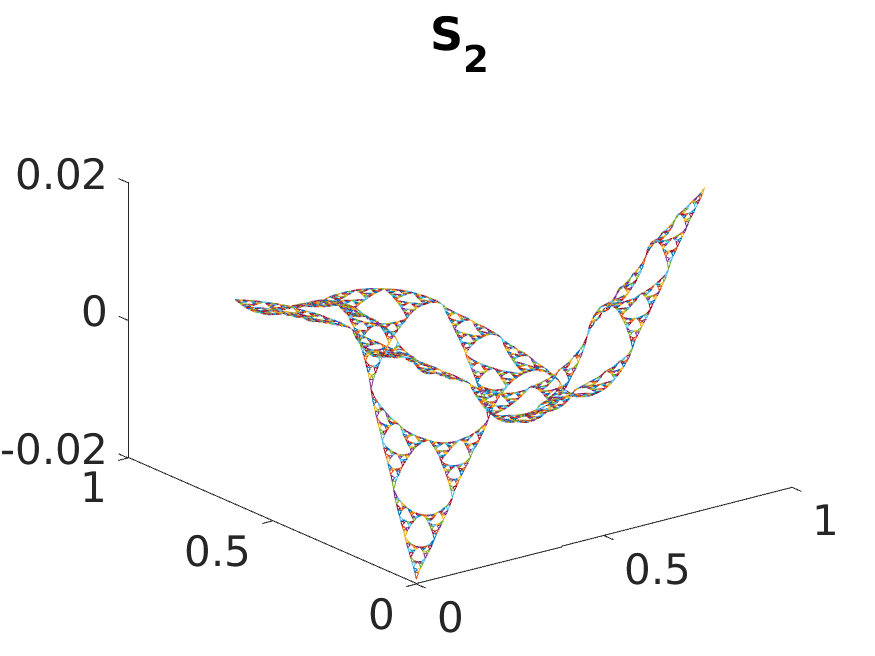
\includegraphics[width=\textwidth]{images/H1AntisymOPs0_23/SAntiSym2.png}
    \end{minipage}
    \begin{minipage}{.3\textwidth}
    \centering
    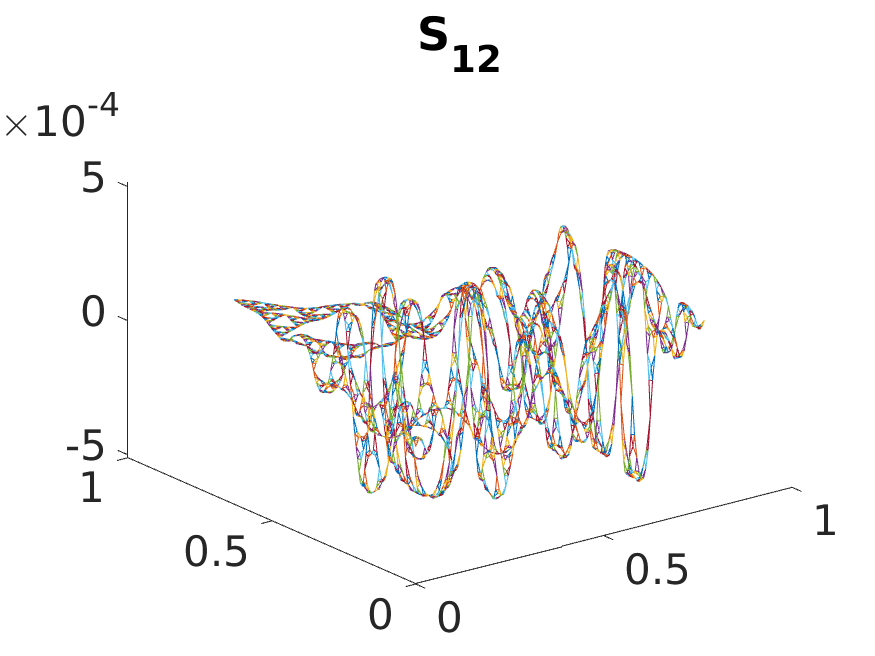
\includegraphics[width=\textwidth]{images/H1AntisymOPs0_23/SAntiSym12.png}
    \end{minipage}
    \begin{minipage}{.3\textwidth}
    \centering
    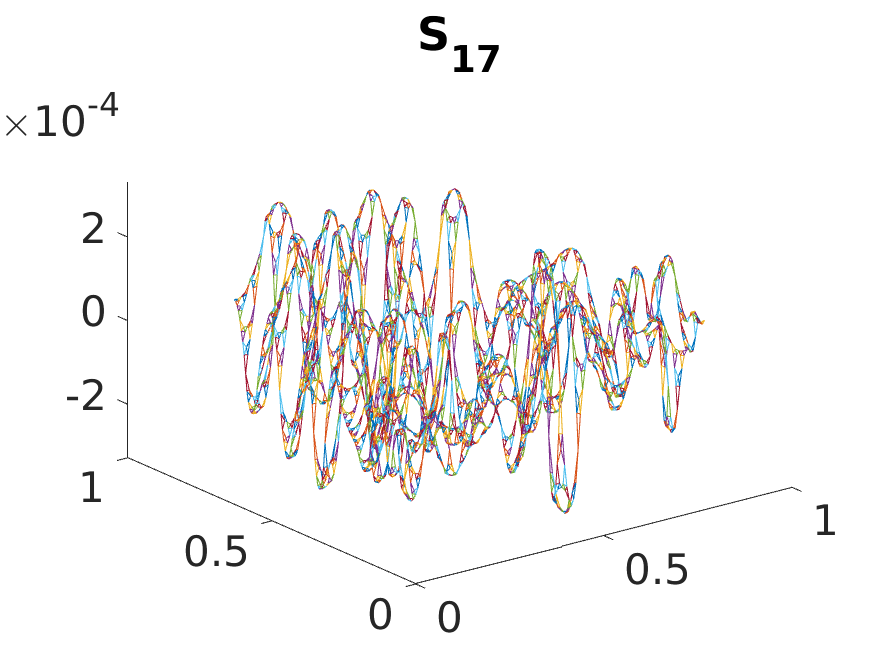
\includegraphics[width=\textwidth]{images/H1AntisymOPs0_23/SAntiSym17.png}
    \end{minipage}
    \begin{minipage}{.3\textwidth}
    \centering
    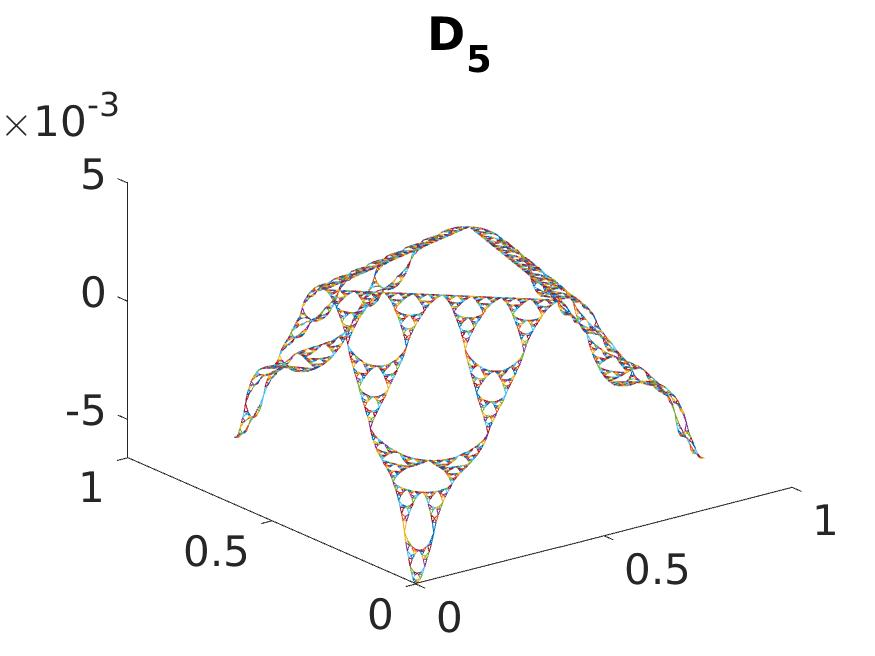
\includegraphics[width=\textwidth]{images/H1SymmOPs0_19/Ss5.jpg}
    \end{minipage}
    \begin{minipage}{.3\textwidth}
    \centering
    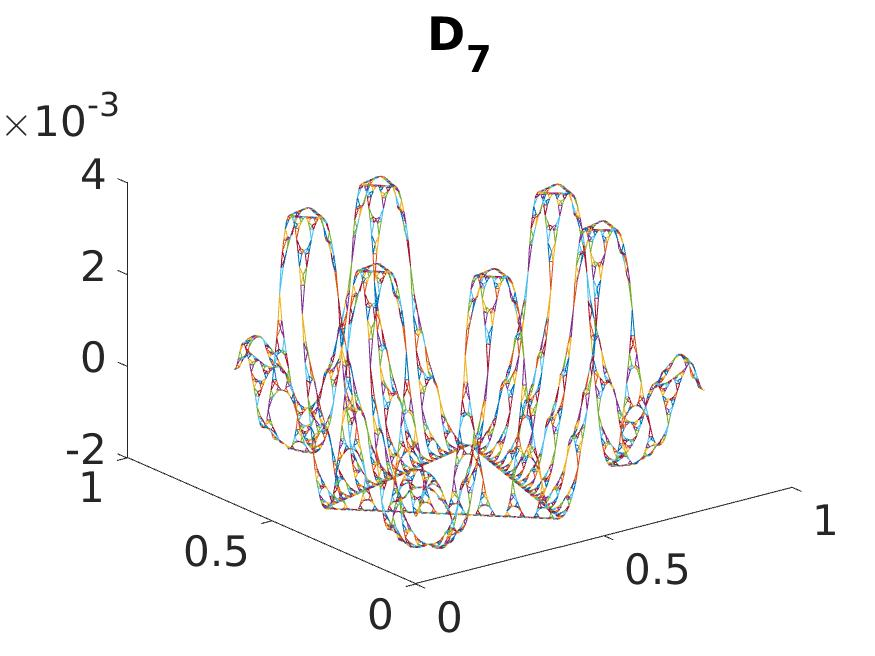
\includegraphics[width=\textwidth]{images/H1SymmOPs0_19/Ss7.jpg}
    \end{minipage}
    \begin{minipage}{.3\textwidth}
    \centering
    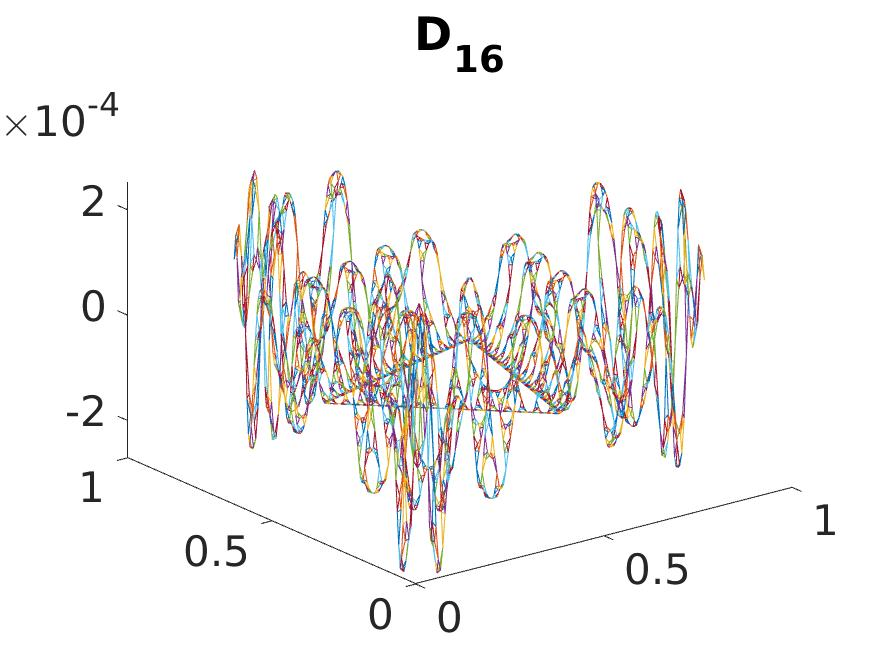
\includegraphics[width=\textwidth]{images/H1SymmOPs0_19/Ss16.jpg}
    \end{minipage}
    
    \caption{Plots of Anti-Symmetric and Symmetric $H^1$ orthonormal polynomials}
    \label{fig: Symmetric and Antisymmetric plots}
\end{figure}

We notice that the Sobolev polynomials are 4 orders of magnitude lower than the Legendre polynomials found in Figure 4 of \cite{OST}. This is due to the $L^{\infty}$ estimate given in Corollary \ref{Corollary: laplacian-L2 and Linfinity estimates}. The estimate also shows that $S_n$ decays to the zero polynomial uniformly as $n \rightarrow \infty$ due to the decay in $\|p_n\|_{L^2}$. 

We were also interested in verifying if the Sobolev-Legendre polynomials on SG exhibited interlacing properties noted for coherent pairs. Let $S_n$ be the orthogonal polynomials with respect to the measure $\mu_0$ and $P_n$ the orthogonal polynomials with respect to the measure $\mu_1$. In \cite{MX} it is stated that if $(d\mu_0, d\mu_1)$ form a coherent pair on $[-1,1]$, then the zeros of the polynomial $S_n$, interlace with those of $P_n$ and $P_{n-1}$. However, on SG, the self-similar measure is not self-coherent but (2,0) self-coherent of order (1,0), and also, the properties of polynomials are quite different. 

\begin{figure}[H]
    \begin{subfigure}{\linewidth}
  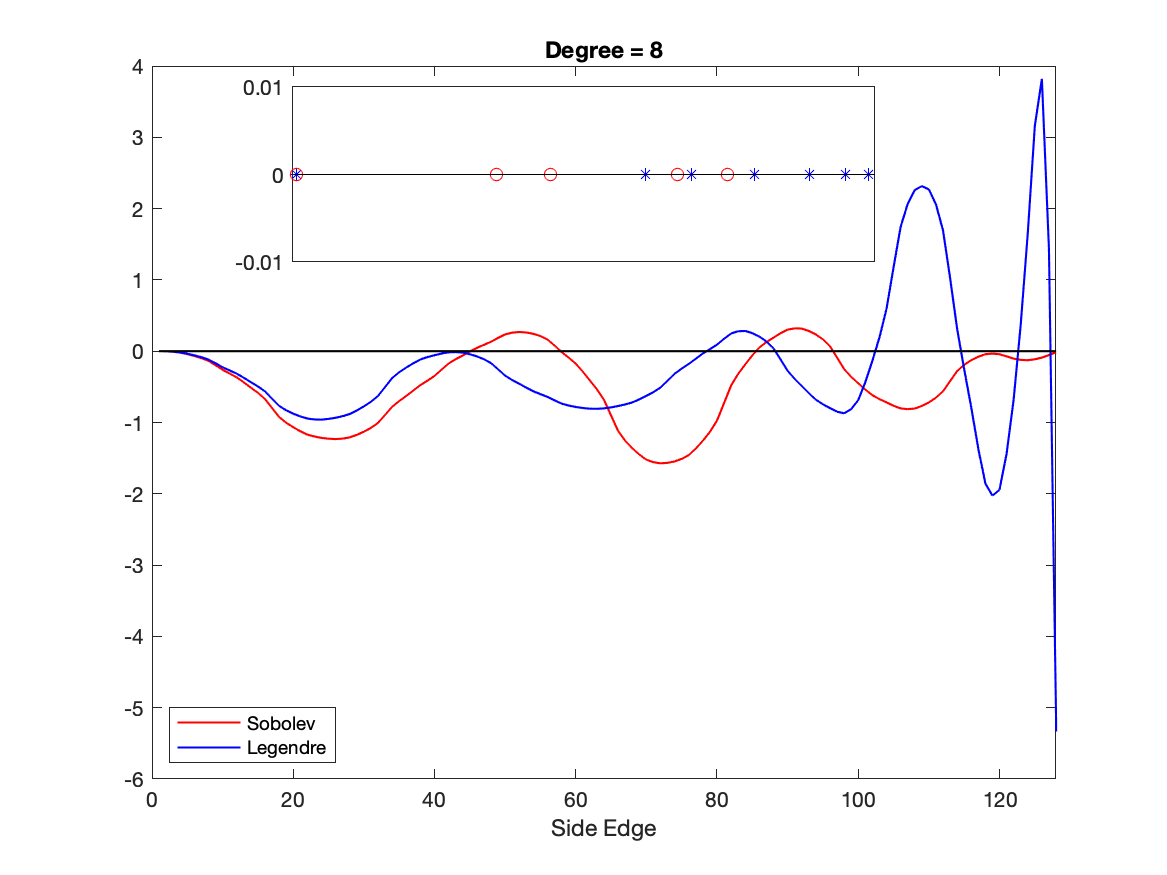
\includegraphics[width=.32\linewidth]{images/LSSEInterlacingAS/ls8.png}
  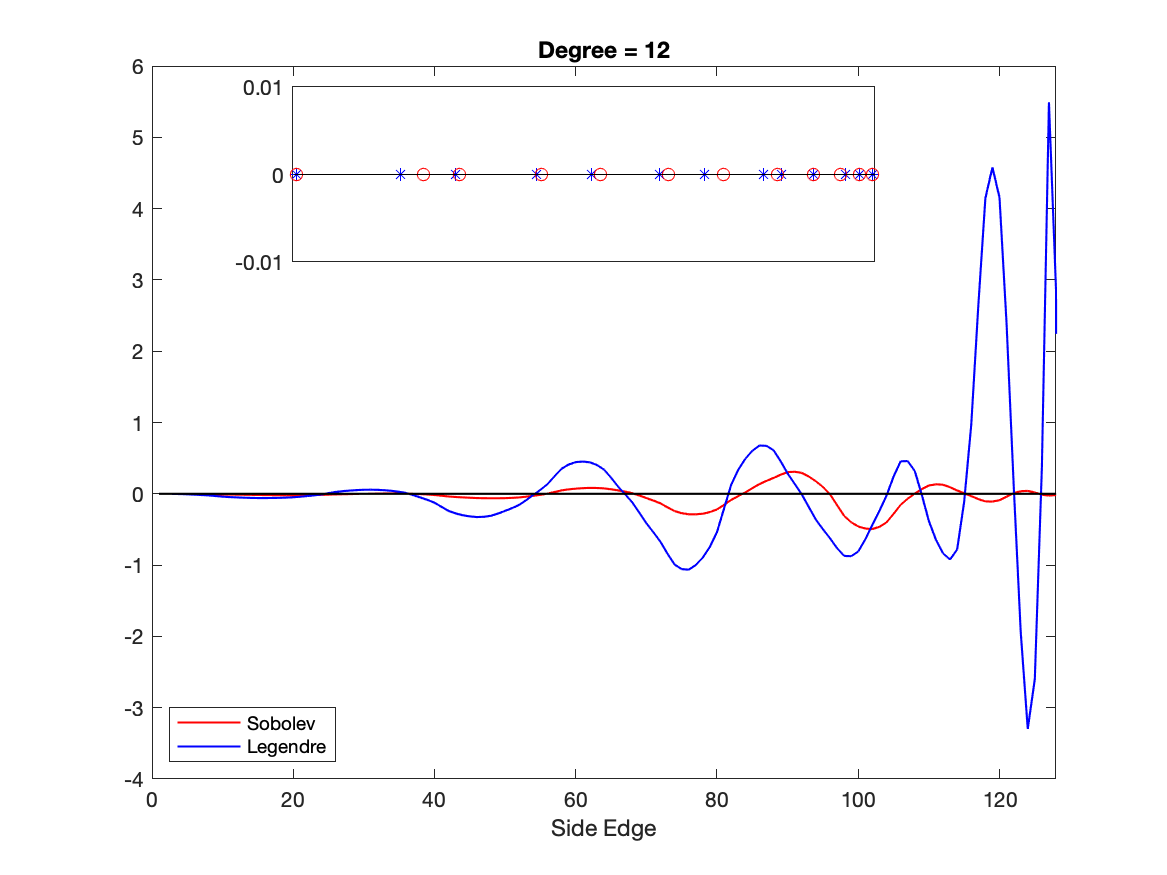
\includegraphics[width=.32\linewidth]{images/LSSEInterlacingAS/ls12.png}
  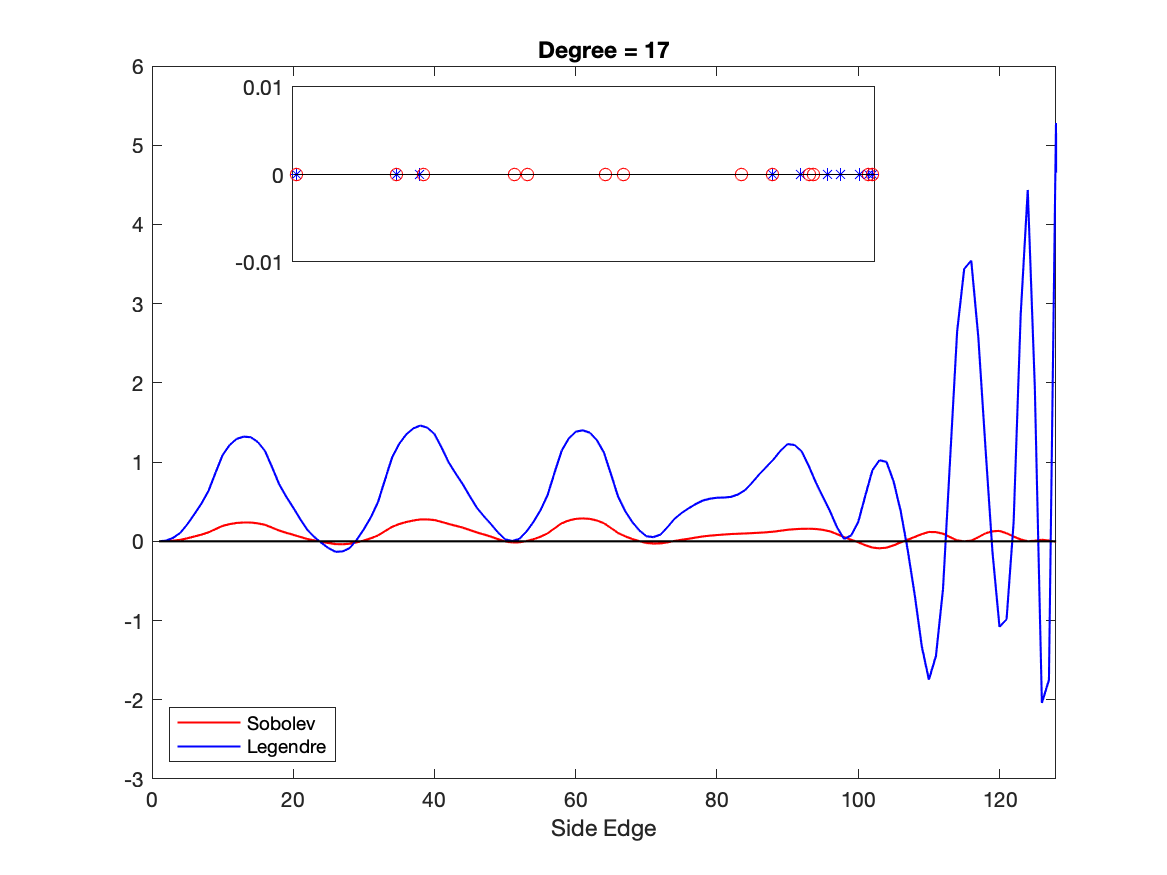
\includegraphics[width=.32\linewidth]{images/LSSEInterlacingAS/ls17.png}
  \caption{Anti-Symmetric Legendre and Sobolev polynomials on the edge between $q_0$ and $q_1$}
  \label{subfig:LSSEinterlacingAS}
  \end{subfigure}\par\medskip
  \begin{subfigure}{\linewidth}
  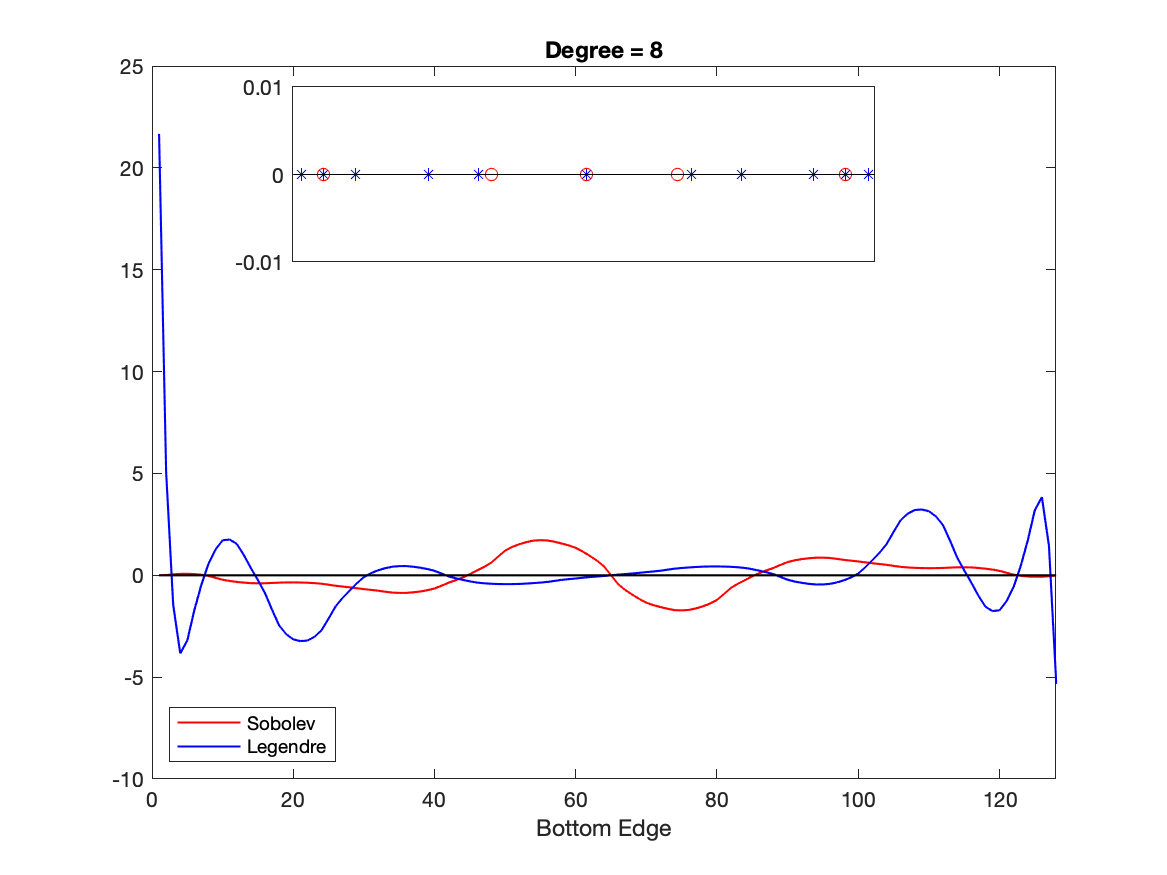
\includegraphics[width=.32\linewidth]{images/LSBEinterlacingAS/ls8.png}
  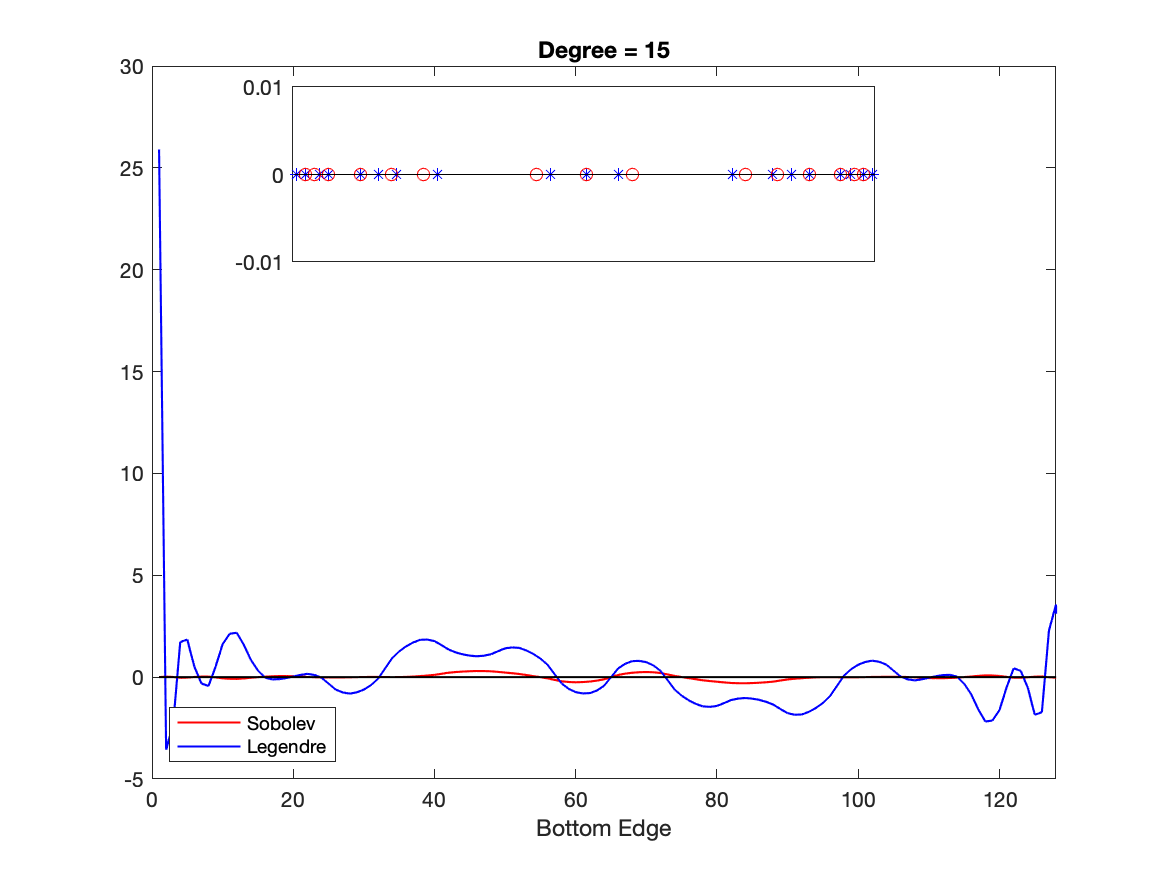
\includegraphics[width=.32\linewidth]{images/LSBEinterlacingAS/ls15.png}
  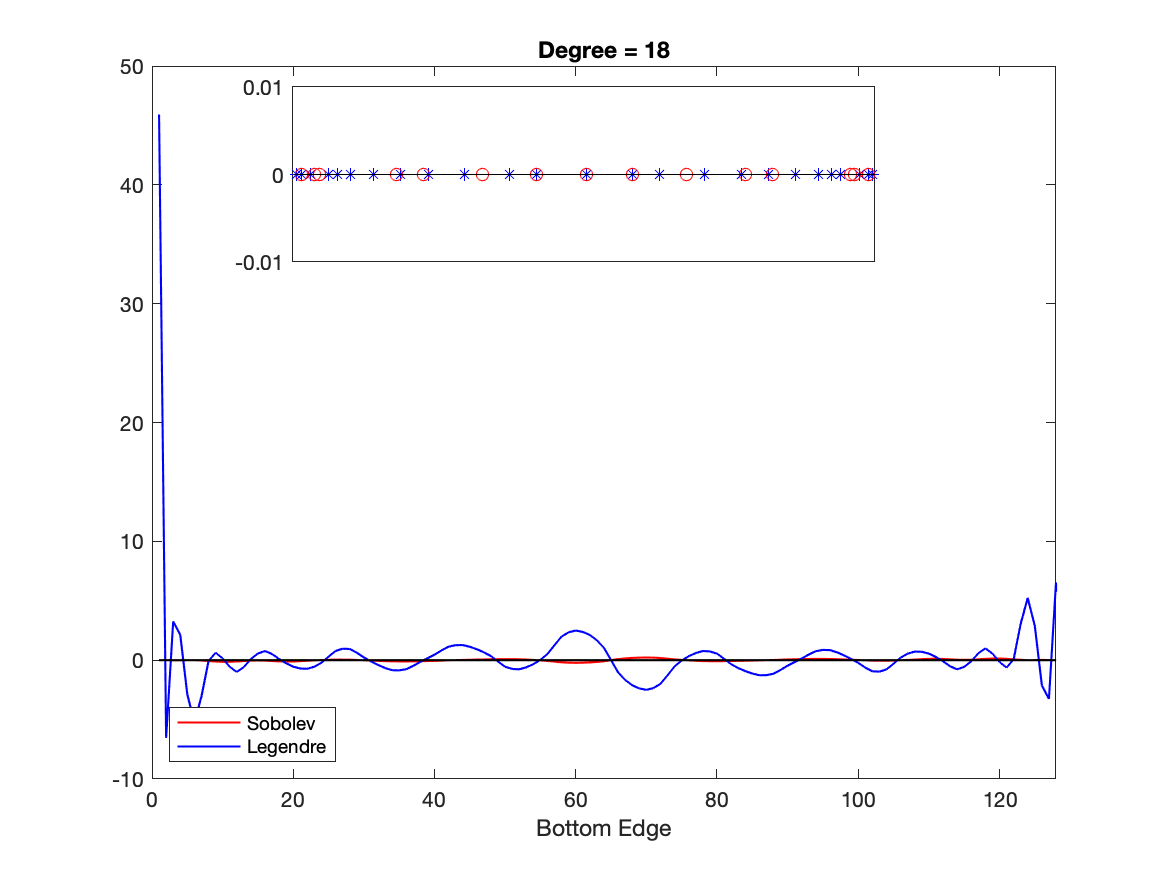
\includegraphics[width=.32\linewidth]{images/LSBEinterlacingAS/ls18.png}
  \caption{Anti-Symmetric Legendre and Sobolev polynomials on the edge between $q_1$ and $q_2$}
  \label{subfig:LSBEinterlacingAS}
  \end{subfigure}\par\medskip
  \begin{subfigure}{\linewidth}
  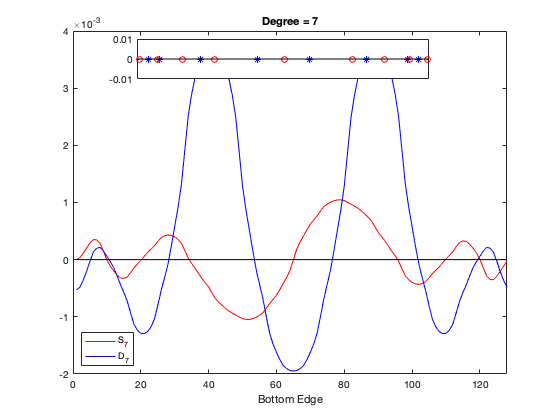
\includegraphics[width=.32\linewidth]{images/SASSBEInterlacing/sd7.png}
  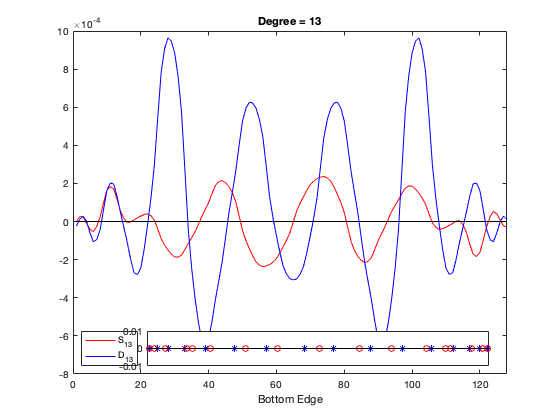
\includegraphics[width=.32\linewidth]{images/SASSBEInterlacing/sd13.png}
  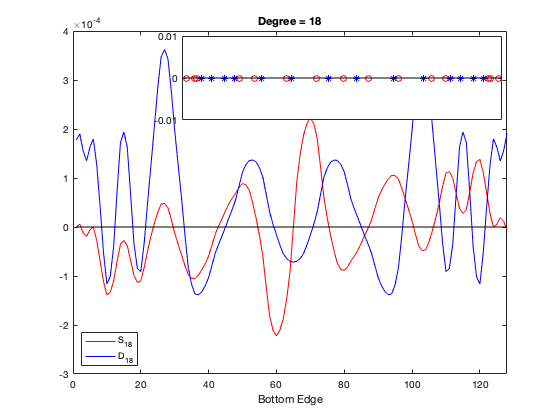
\includegraphics[width=.32\linewidth]{images/SASSBEInterlacing/sd18.png}
  \caption{Symmetric and Anti-symmetric Sobolev polynomials on the edge between $q_1$ and $q_2$}
  \label{subfig:SASSBEinterlacing}
  \end{subfigure}
  \caption{Interlacing patterns of $S_n$, $D_n$, and $p_n$ on the edges of SG}
  \label{fig: Interlacing}
\end{figure}

Figure \ref{fig: Interlacing} reveals that such mutual interlacing patterns between $p_n$, $S_n$ are highly irregular on the edges of SG. Furthermore, \ref{subfig:LSBEinterlacingAS} suggests that the zeros of $S_n$ may not all be simple: $S_17$ seems to have a zero of multiplicity greater than one. However, this is difficult to prove analytically: we can use data at higher resolutions to lend credence to this guess. Finally, we take a look at the number of zeros of the polynomials: 

\begin{figure}[H]
    \centering
    \begin{subfigure}{\linewidth}
    \centering
    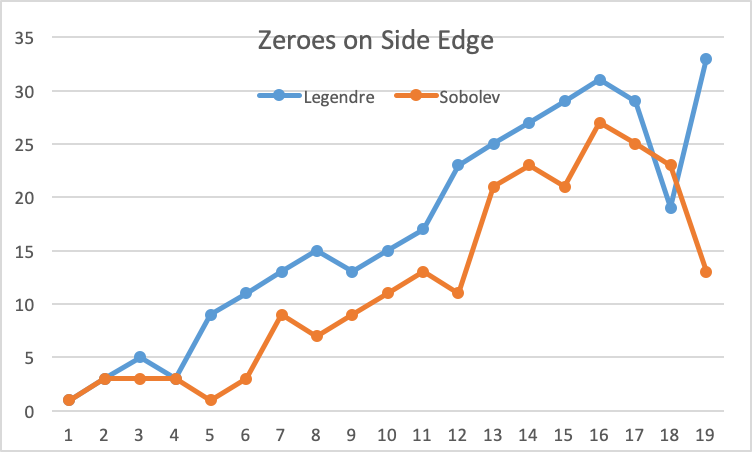
\includegraphics[width=0.65\linewidth]{images/SEzeroes.png}
    \caption{Zeros on Side edges}
    \label{subfig:zerosonsideedgeantisymmetric}
    \end{subfigure}
    \begin{subfigure}{\linewidth}
    \centering
    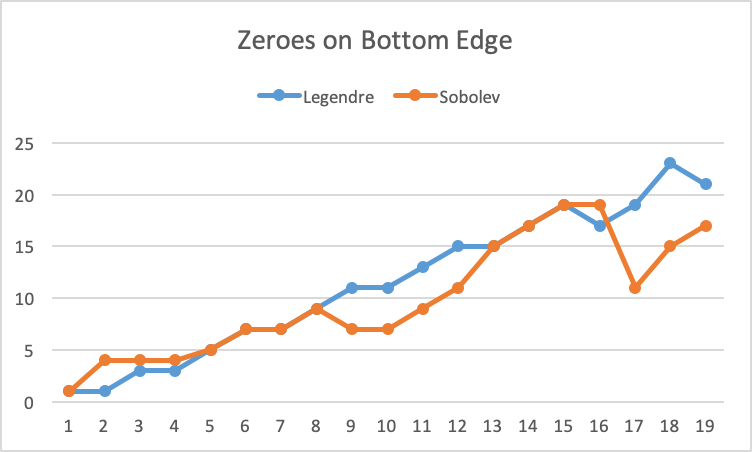
\includegraphics[width=0.65\linewidth]{images/BEzeroes.png}
    \caption{Zeros on Bottom edge}
    \label{subfig:zerosonbottomedgeantisymmetric}
    \end{subfigure}
    \begin{subfigure}{\linewidth}
    \centering
    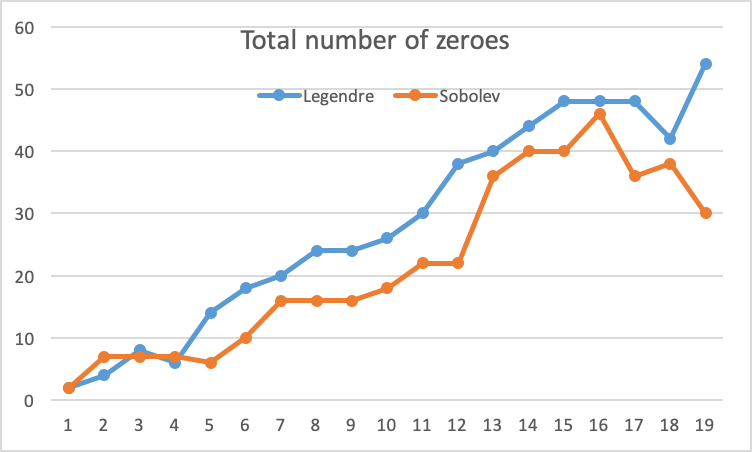
\includegraphics[width=0.65\linewidth]{images/TotalZeroes.png}
    \caption{Total number of zeros on the edges}
    \label{subfig:zerostotalantisymmetric}
    \end{subfigure}
    \caption{Comparison of number of zeros between the Anti-Symmetric Legendre and Sobolev orthogonal polynomials on the edges}
    \label{fig: edgezeros}
\end{figure}

\begin{table}[H]
\centering
\caption{Number of zeroes of $S_n$ and $p_n$ up to $n=18$ on the edges}
\begin{tabular}{*7c}
\toprule
Degree &  \multicolumn{3}{c}{Legendre ($p_n$)} & \multicolumn{2}{c}{Sobolev ($S_n$)}\\
\midrule
 {}& Bottom Edge & Side Edges & Total & Bottom Edge & Side Edges & Total \\
	0 & 1 & 1 & 2 & 1 & 1 & 2 \\ 
	1 & 1 & 3 & 4 & 4 & 3 & 7 \\ 
	2 & 3 & 5 & 8 & 4 & 3 & 7 \\
	3 & 3 & 3 & 6 & 4 & 3 & 7 \\  
	4 & 5 & 9 & 14 & 5 & 1 & 6 \\  
	5 & 7 & 11 & 18 & 7 & 3 & 10 \\  
	6 & 7 & 13 & 20 & 7 & 9 & 16 \\  
	7 & 9 & 15 & 24 & 9 & 7 & 16 \\  
	8 & 11 & 13 & 24 & 7 & 9 & 16 \\  
	9 & 11 & 15 & 26 & 7 & 11 & 18 \\  
	10 & 13 & 17 & 30 & 9 & 13 & 22 \\  
	11 & 15 & 23 & 38 & 11 & 11 & 22 \\  
	12 & 15 & 25 & 40 & 15 & 21 & 36 \\  
	13 & 17 & 27 & 44 & 17 & 23 & 40 \\  
	14 & 19 & 29 & 48 & 19 & 21 & 40 \\  
	15 & 17 & 31 & 48 & 19 & 27 & 46 \\  
	16 & 19 & 29 & 48 & 11 & 25 & 36 \\  
	17 & 23 & 19 & 42 & 15 & 23 & 38 \\  
	18 & 21 & 33 & 54 & 17 & 13 & 30 \\  
\bottomrule
\end{tabular}
\label{table: antisymmetric zeroes}
\end{table}

Once again, the pattern of zeros on the edges is irregular. While number of zeros is generally monotonic, there are some exceptions, such as $p_{18}$ or $S_5$, which have fewer zeros overall than their lower-degree counterparts. Actually, this is a clear difference from the case on $[-1,1]$ where both the Sobolev and Legendre polynomials have exactly $n$ zeros. 

\begin{remark}\label{remark:methodology in zeroes}
By the bottom edge, we mean the edge between $q_1$ and $q_2$ included. By a side edge, we mean the edge between $q_0$ and $q_i$ for $i=1,2$ including $q_0$ but not $q_i$ Our methodology in counting zeroes was rudimentary. We plotted the polynomials on $\Gamma_7$, which meant we had $129$ evaluation points on each edge. Then we simply computed the number of times the polynomial changed sign and concluded that by continuity the polynomial must have had a zero in the interval. There are two clear issues with this methodology: first, the polynomial may have more than one zero between two points of opposite sign. Secondly, this methodology cannot be used to compute non-simple zeroes. From the plots we observe that the edges look tangential to the polynomials at some points, implying the existence of high-multiplicity zeroes (HMZs). But we can only evaluate the polynomial at finitely many points. Consequently, sometimes, an HMZ can get trapped between evaluation points, so in our data it looks like the polynomial takes a non-zero value at the HMZ. 
\end{remark}

\begin{remark}\label{remark: Further challenges}
The complete set of data can be found at \cite{[JSV]}. We suggest the following courses of further action:

\begin{enumerate}
    \item Identifying polynomial behaviour on the fundamental triangle
    \item Plotting nodal domains as done in \cite{OST}
    \item Collecting higher resolution, high degree data
    \item Repeating the above experiments for different values of $\lambda$ (although the result in \ref{Corollary: Convergence result for lambda} tells us what the $H^1$ polynomials should start behaving like)
    \item Plot the coefficients $a_n$ and $b_n$ appearing in the recurrence.
    \item Repeat the above experiments for the other types of Sobolev inner products mentioned in \ref{remark: Other kinds of $H^1$ inner product}. 
    \item Derive an orthonormal system $\phi_n$ from $S_n$ and $D_n$ and repeat above experiments. 
\end{enumerate}

We suggest doing these in Python3 instead of Matlab, due to a mutation issue in the data files.
\end{remark}

\subsection{Polynomial Interpolation}

We begin this subsection with an examination of Table \ref{table: antisymmetric zeroes}, which counts the zeroes of the anti-symmetric Legendre and Sobolev polynomials, denoted $p_n$ and $S_n$ respectively. First of all, $p_n$ and $S_n$ are anti-symmetric, so we need only look at their zeroes on one of the halves of SG separated by the line passing through $F_1q_2$ and $q_0$, referred to henceforth as $l_0$. Consider the case of $S_{15}$. $S_{15}$ has 19 zeroes in total on the bottom edge, which means it has $9$ zeroes strictly in the left half of the bottom edge. It has 27 total side edge zeroes, implying that it has $13$ zeroes strictly between $q_0$ and $q_1$. Thus, it has at least 22 zeroes in one half that do not lie on $l_0$. Let $x_0, \ldots x_{15}$ represent the first 16 of these zeroes. Then our observation is equivalent to saying that the matrix

\begin{align}
    \begin{bmatrix}
    P_{0,3}(x_0) & \ldots & P_{15,3}(x_0) \\
    \vdots & \ddots & \vdots \\
    P_{0,3}(x_{15}) & \ldots & P_{15,3}(x_{15})\\
    \end{bmatrix}
\end{align}

is not invertible. This statement is in stark contrast with polynomials on $\RR$ because the fundamental theorem of algebra implies that the values of an $n$-degree polynomial on $n+1$ distinct points determines the polynomial. On $SG$, a polynomial $f$ of degree $n$ is given as 

$$ f(x) = \sum_{j=0}^{n}\sum_{k=1}^{3}c_{j,k}P_{j,k}(x)$$

The corresponding question on $SG$ is then called the $\textit{interpolation problem on SG}$:

\begin{question}
Does sampling an $n$ degree polynomial on any $3n + 3$ points uniquely determine the polynomial? 
\end{question}

Answer: No! We have the counter-example of $S_{14}$. For the remainder of this section we consider the following problem: 

\begin{problem}\label{prob: Interpolation problem}
At which points $x_1, \ldots, x_{3n+3}$ is the matrix 

\begin{align}\label{interpolationmatrix}
    M_n = \begin{bmatrix}
    P_{0,1}(x_1) & \ldots & P_{n,3}(x_1) \\
    \vdots & \ddots & \vdots \\
    P_{0,1}(x_{3n+3}) & \ldots & P_{n,3}(x_{3n+3})\\
    \end{bmatrix}
\end{align}

invertible? 
\end{problem}

Here $M_n$ is termed as the interpolation matrix on the set $\{x_1, \ldots, x_n\}$. There is no clear answer to the above problem. However, there are some obviously poor choices of points. For example, if we take $x_i=F_0^{(i-1)}(q_1)$ with $1\le i \le3n+3$,  then $[P_{1,1}(x_1)\ldots P_{1,1}(x_{3n+3})]$ is parallel to $[P_{0,3}(x_1)\ldots P_{0,3}(x_{3n+3})]$ by scaling properties, hence definitely the matrix will not be invertible. Also if we restrict ourselves to the space of anti-symmetric polynomials then Problem \ref{prob: Interpolation problem} is changed to checking the invertibility of 

\begin{align}
    \begin{bmatrix}
    P_{0,3}(x_1) & \ldots & P_{n,3}(x_1) \\
    \vdots & \ddots & \vdots \\
    P_{0,3}(x_{n+1}) & \ldots & P_{n,3}(x_{n+1})\\
    \end{bmatrix}
\end{align}

In this case, we would rather not select some $x_i$ to be the reflection of some other point $x_j$ because then two rows of the matrix become linearly dependent. The same is true for polynomials in the symmetric space spanned by $\{P_{j,1}, P_{j,2}\}$. We do, however, have the following lemma: 

\begin{lemma}
Let $g \in \mathcal{H}_1$. Then $g$ is determined uniquely by its values on $V_1$
\end{lemma}

\begin{proof}
The proof is by direct computation of the interpolation matrix. We switch to the easy basis $\{f_{jk}\}$ where $j=0,1$ and $k=0,\ldots,2$. Suppose $g|_{V_0} \equiv 0$. Then, $g = c_0f_{10} + c_1f_{11} + c_2f_{12}$. Now suppose $g|_{V_1} \equiv 0$. Then to check whether $c_i = 0$ we need to check the invertibility of

$$ \begin{bmatrix}
f_{10}(F_0q_1) & f_{11}(F_0q_1) & f_{12}(F_0q_1) \\
f_{10}(F_1q_2) & f_{11}(F_1q_2) & f_{12}(F_1q_2) \\
f_{10}(F_2q_0) & f_{11}(F_2q_0) & f_{12}(F_2q_0)\\
\end{bmatrix}$$

But this is a circulant matrix and $f_{10}(F_0q_1) + f_{11}(F_0q_1) + f_{12}(F_0q_1) = -1/15 \neq 0$ so it is invertible. 

\end{proof}

\begin{remark}\label{rem:circulant}
We may attempt to generalize the above proof since $\forall j \geq 0$, $f_{jk}(\rho x) = f_{j\rho^2(k)}(x)$ where $\rho$ rotates $SG$ counterclockwise by $2\pi/3$ (assume $q_0\rightarrow q_1\rightarrow q_2$ is counterclockwise direction), or equivalently, corresponds to the permutation $(1 2 3)$. Thus, if we first select points $x_0, \ldots x_{n}$ and then complete the rest of the set by taking $\rho(x_i)$ and $\rho^2(x_i)$ then the interpolation matrix $M_n$ can be expressed as a circulant-block matrix: 

$$ M_n = \begin{bmatrix}
C_{0,0} & \hdots & C_{0,n} \\
\vdots & \ddots & \vdots \\
C_{n,0} & \hdots & C_{n,n}\\
\end{bmatrix}$$

where 

$$C_{i,j} = \begin{bmatrix}
f_{j,0}(x_i) & f_{j,1}(x_i) & f_{j,2}(x_i)\\
f_{j,0}(\rho(x_i)) & f_{j,1}(\rho(x_i)) & f_{j,2}(\rho(x_i))\\
f_{j,0}(\rho^2(x_i)) & f_{j,1}(\rho^2(x_i)) & f_{j,2}(\rho^2(x_i))\\
\end{bmatrix} = \begin{bmatrix}
f_{j,0}(x_i) & f_{j,1}(x_i) & f_{j,2}(x_i)\\
f_{j,2}(x_i) & f_{j,0}(x_i) & f_{j,1}(x_i)\\
f_{j,1}(x_i) & f_{j,2}(x_i) & f_{j,0}(x_i)\\
\end{bmatrix} $$

We have not yet been able to prove that $M_n$ is invertible in general. In the case $n=2$, we can prove invertibility by using Schur complement to invert the matrix. When $n=2$, the Schur complement itself turns out to be circulant invertible. However, for larger $n$ this proof strategy does not work. We computed the determinants of $M_n$ for larger values of $n$ and found that they were all non-zero. The points we used were: $x_0 = q_1$, $x_i = F^{i}_{1}(q_0)$ and their rotations. 
\end{remark}
Fortunately, we have one solution for Problem \ref{prob: Interpolation problem}.
\begin{lemma}\label{lemma:solinterpolation}
For any $n\ge 0$, take $x_i=F_0^{(i-1)}(q_1)$ for $1\le i\le 2n+2$, and $x_i=F_0^{(i-2n-3)}(q_2)$ for $2n+3\le i \le 3n+3$. Then the matrix \eqref{interpolationmatrix} is invertible.
\end{lemma}
\begin{proof}
Suppose not, then there exists a  non-zero vector $[\alpha_1\ldots\alpha_{3n+3}]$ such that $f(x_i)=0$ for any $i$, with $f:= \sum\limits^{i=n+1}_{i=1}\alpha_iP_{i-1,1}+\alpha_{n+1+i}P_{i-1,2}+\alpha_{2n+2+i}P_{i-1,3}$. Note $f(F_0^{(i-1)}(q_1))=f(F_0^{(i-1)}(q_2))=0$ for $1\le i \le n+1$. By symmetry, we have $f_0(F_0^{(i-1)}(q_1))=0$ for $1\le i \le n+1$, where $f_0:=\sum\limits^{i=n+1}_{i=1}\alpha_{2n+2+i}P_{i-1,3}$. But notice the determinant of
$\begin{bmatrix}
    P_{0,3}(x_1) & \ldots & P_{n,3}(x_1) \\
    \vdots & \ddots & \vdots \\
    P_{0,3}(x_{n+1}) & \ldots & P_{n,3}(x_{n+1})
\end{bmatrix}$
is the product of some $\gamma_i$ (which is positive) and the determinant of a Vandermonde Matrix, which is $\prod\limits_{1\le i<j\le n+1}(5^{-j}-5^{-i})$ (by the scaling property). It follows that $f_0=0$. Now we consider $f_1:=f-f_0$, by similar argument and use determinant of Vandermonde Matrix (notice $5^{-j}\neq 5^{-i}$ if $i\neq j$, and $\frac35 5^{-i}\neq 5^{-j}$ for any $i,j$). One particular point we should pay attention to is to prove $\beta_j\neq0$, notice by Theorem 2.9 in \cite{NSTY}, $(-\lambda_2)^j\beta_j$ will converge to a non-zero value as $j\rightarrow\infty$, where $\lambda_2=135.572126995788...$. Moreover the rate of convergence can be estimated so that it suffices to verify the cases when $j$ is small. Hence we have $f=f_1=0$ and a contradiction arises.\end{proof}
\begin{definition}
Let $I_n \subseteq SG$. Then $I_n$ is termed an $n$-interpolatory set of $SG$ if for any subset $N \subseteq I$ such that $|N| = 3n + 3$, $M_n$ is invertible on $N$.
\end{definition}

Note that the set proposed in Lemma \ref{lemma:solinterpolation} is $n$-interpolatory since it has exactly one subset of $3n + 3$ elements: itself. Furthermore, $M$ is invertible on this set so it is $n$-interpolatory. The set of zeroes of $p_{12}$ is not $12$-interpolatory because it contains a set of $39$ points where $M_n$ is non-invertible. We deploy a trick of Haar to show that measurable $n$-interpolatory sets have measure 0. 

\begin{proposition}
Let $I_n \subseteq SG$ be an $n$-interpolatory set. Then $I_n$ cannot contain a cell with $3n + 1$ additional points.
\end{proposition}

\begin{proof}
Suppose there is a cell $C$ such that $C \in I_n$. Then pick $I = \{a,b\}$ a set of 2 junction points $a$ and $b$ strictly in the interior. Now there exist two paths $\gamma$ and $\eta$ joining $a$ and $b$ such that they are disjoint except at the endpoints. Pick $B = \{x_1, \ldots x_{3n + 1}\}$, a set of any $3n + 1$ points not on $\gamma \cup \eta$. Thus, $S = B \cup I$ is a set of $3n + 3$ points and so $M_n$ is invertible on $S$ since $I_n$ is $n$-interpolatory. We may parametrize the paths $\gamma$ and $\eta$ as $\gamma(t)$ and $\eta(t)$ where $0 \leq t \leq 1$ such that $\gamma(1) = \eta(0) = a$ and $\gamma(0) = \eta(1) = b$. Now for every $t$, $M_n$ $\{\eta(t),\gamma(t)\} \cup B$ stays invertible as we picked $B$ to not coincide with $\gamma$ and $\eta$. Traversing the two paths from $t=0$ to $t=1$ switches the rows of $M_n$ and hence the sign of its determinant. However, the determinant is a continuous function of $t$ since it is a polynomial of the monomials composed with $\gamma$ and $\eta$ which are themselves continuous. Thus, the determinant changes sign in the interval $[0,1]$ and hence by IVT must be 0 for some $T \in (0,1)$. Consequently, $M_n$ is not invertible in the set $B \cup \{\gamma(T), \eta(T) \} \subseteq I_n$, which is a contradiction since we assumed $I_n$ was $n$-interpolatory.
\end{proof}

As a corollary we have that measurable interpolatory sets cannot contain cells which means they have measure 0. As of now, we have not found any non-measurable interpolatory sets. 

\subsection{Quadrature on SG}
One of the most important applications of orthogonal polynomials is in developing quadrature and interpolation rules. Due to properties of their inner products, orthogonal polynomials on the real line can be used to develop highly efficient quadrature rules. For example, we consider the case of Gauss-Legendre quadrature. The goal of a polynomial quadrature rule is to be able to integrate a degree $n$ polynomial exactly. Then, by approximating a given function by degree $n$ splines, we approximate its integral. Normally, by knowing the exact integral of a degree $n$ polynomial, we are able to only use polynomials up to degree $n$ in the approximation of our function. However, if we choose a Legendre orthogonal polynomial of degree $n$, we find that we will be able to use polynomials up to degree $2n+1$ in the approximation of our function.

Consider a polynomial $f$ of degree $2n+1$ and let $p_{n+1}$ be the degree $n+1$ Legendre polynomial. Since we have a polynomial division algorithm on the real line, we can write $f = qp_{n+1} + r$ where $\deg q, r \leq n$. Then
\begin{align}\label{eq:polydiv}
    \int f\cdot w = \int p_{n+1}q \cdot w+ \int r\cdot w = \int r\cdot w
\end{align}
where the last equality is due to the fact that $p_{n+1}$ is orthogonal to all lower degree polynomials. So, if we choose the quadrature nodes to be the roots of $p_{n+1}$, we have the quadrature rule
\begin{align}\label{eq:gaussquad}
    \int r\cdot w = \sum f(x_i) \int l_i\cdot w = \sum f(x_i) w_i
\end{align}
where $l_i$ is the $i^{\textrm{th}}$ Lagrange interpolating polynomial for the roots of $p_{n+1}$ and $w_i = \int l_i \cdot w$. Thus, by using polynomial division, we gain a massive increase in the precision of our quadrature. 

On SG, we do not have the luxury of a true polynomial division algorithm. Since the domain of the Laplacian on SG does not form an algebra, the product of two nontrivial polynomials is no longer a polynomial. We do observe a method for quasi-polynomial-division as follows:

\begin{remark}\label{rem:SGdivision}
Suppose $f$ and $g$ are polynomials of degree $n$ and $m$ respectively on SG (with $n \geq m$) from the same family ($k = 1, 2,$  or $3$). write $f = \sum\limits_{i = 0}^n a_iP_{ik}$ and $g = \sum\limits_{j=1}^m b_jP_{jk}$. Then we can define the quotient operator $\mathcal{Q}_f$ and remainder $r$ when we divide $f$ by g:
    \begin{align}\label{eq:SGdivision}
        \mathcal{Q}_f &= \frac{1}{b_m}
        \sum\limits_{i = 0}^{n-m}c^{(i)}\mathcal{G}^{(n-m-i)}\\
        r &= f - \mathcal{Q}_fg
    \end{align}
where $c^{(i)}$ is so that we have $f = Q_fg + r$ and $0 < \deg r < m$ or $r$ is harmonic.
\end{remark}
We see that on SG, since we do not have true polynomial division, we cannot fully replicate the Gauss-Legendre quadrature algorithm on $\RR$.

Without Gauss-Legendre quadrature, our next best approach is to find an algorithm to use n-Harmonic splines for quadrature. In this case, we write $\int f \approx \sum\limits_i f(x_i)w_i$ so that we can exactly integrate up to n-Harmonic functions. We arrive at the following system of equations

\begin{align}\label{eq:interpol}
    \begin{bmatrix}
    P_{1}(x_1) & P_{1}(x_{2}) & \dots & P_{1}(x_{3n+3})\\
    \vdots & \vdots & \ddots & \vdots \\
    P_{3n+3}(x_{1}) & P_{3n+3}(x_{2}) & \dots & P_{3n+3}(x_{3n+3})
    \end{bmatrix}
    \begin{bmatrix}
    w_1\\
    \vdots\\
    w_{3n+3}
    \end{bmatrix} = 
    \begin{bmatrix}
    \int_{SG}P_{1}\\
    \vdots\\
    \int_{SG}P_{3n+3}
    \end{bmatrix}
\end{align}
where $P_j$ are any set of $3n+3$ monomials forming a basis for $\mathcal{H}_n$. Thus, we see that the solvability of \ref{eq:interpol} is equivalent to solving the interpolation problem on SG (\ref{prob: Interpolation problem}).

Experimentally, we see that the interpolation matrices $M_n$ constructed in Remark \ref{rem:circulant} have non-zero determinant for at least $n \leq 50$ in exact rational precision.

We observe that many of the outstanding problems regarding polynomials in SG can be solved by determining an n-Harmonic extension algorithm. On SG, it is possible to extend a function defined on the boundary set $V_0$ harmonically using the $\frac15-\frac25$ rule. The goal of an n-Harmonic extension algorithm would be to extend a function defined on $3n+3$ specific vertices in $V_m$ n-Harmonically. Given such an algorithm, we would be able to solve the interpolation problem (\ref{prob: Interpolation problem}) and obtain the following estimate for an n-Harmonic spline quadrature rule:

\begin{theorem}

\label{thm:nharmquad}
Suppose we have a solution to the interpolation problem (\ref{prob: Interpolation problem}) and a quadrature rule $I_n^n(f):=\sum\limits_{i=1}^{3n+3}\omega_if(x_i)$ which exactly integrates functions in $\mathcal{H}_n$. Let $I_n^m(f):=\sum\limits_{|\omega|=m-n}I^n_n(f\circ F_\omega)$. Then we have the following estimate on the quadrature error:
\begin{align}
    \left|I_n^m(f) - \int_{SG}f\right|\leq c_1(n)5^{-(n+1)m}\|\Delta^{(n+1)}f\|_\infty
\end{align}
In particular it is valid for the chosen points in Lemma \ref{lemma:solinterpolation}.
\end{theorem}


\begin{proof}
Break up $\int_{SG}f$ into integrals over cells $F_wSG$ where $|w| = m-n$. For one such cell, let $g_\omega\in \mathcal{H}_n$ be such that $g_\omega = f\big\rvert_{V_n}$. Then we have
\begin{align}
    \left|I_n^n(f\circ F_w) - \int f\circ F_w\right| =  \left|\int g_\omega - f\circ F_w\right|\\ \leq \|g_\omega - f\circ F_w\|_\infty \leq c_1(n)\|\Delta^{(n+1)}(f\circ F_w)\|_\infty
\end{align}
where the last equality results from applying $(n+1)$-times green operators to $\Delta^{(n+1)}(f\circ F_w)$ and making use of the interpolation and basic properties of finite-dimensional normed space. Combining the subintegrals over the cells and applying the triangle inequality results in
\begin{align}
     \left|I_n^m(f) - \int_{SG}f\right| = 3^{-(m-n)} \left|\sum\limits_{|w| = m-n} I_n^n(f\circ F_w) - \int f\circ F_w\right|\\
     \leq c_1(n)\sup\limits_\omega\|\Delta^{(n+1)}(f\circ F_w)\|_\infty \leq c_1(n)5^{-(n+1)m}\|\Delta^{(n+1)}f\|_\infty
\end{align}

\end{proof}


\begin{section}{Outstanding questions}
We have the following remaining problems: 
\begin{enumerate}
    \item Conjecture \ref{conjecture:normal}
    \item $P_{j1} > 0$ except at $q_0$
    \item Problem \ref{prob: Interpolation problem}
    \item Exploring the questions laid out in remark \ref{remark: Further challenges}. 
\end{enumerate}
\end{section}

\printbibliography
\end{document}
